% ============================================================
%  Preparatório OBI — Aula 04
%  Grafos: Representação, BFS, DFS, Dijkstra e Clássicos
%  Grupo: GEMA
%  Compilar: pdflatex aula04_grafos.tex  (2x para refs)
% ============================================================
\documentclass[aspectratio=169,10pt]{beamer}

\usetheme{Madrid}
\usecolortheme{default}

% ── Pacotes ───────────────────────────────────────────────
\usepackage[utf8]{inputenc}
\usepackage[T1]{fontenc}
\usepackage[english]{babel}
\usepackage{graphicx}
\usepackage{listings}
\usepackage{xcolor}
\usepackage{tikz}
\usepackage{amsmath}
\usepackage{tcolorbox}
\usepackage{array}
\usepackage{booktabs}
\usepackage{adjustbox}
\tcbuselibrary{skins,breakable,listings}
\usetikzlibrary{arrows.meta,shapes,positioning,fit,calc,
                decorations.pathreplacing,backgrounds}

% ── Margens apertadas ─────────────────────────────────────
\setbeamersize{text margin left=4mm,text margin right=4mm}
\setlength{\leftmargini}{1.0em}
\setlength{\leftmarginii}{0.9em}

% ── Paleta de cores ───────────────────────────────────────
\definecolor{gemaBlue}   {RGB}{13,  43,  90}
\definecolor{gemaCyan}   {RGB}{0,  170, 210}
\definecolor{gemaRed}    {RGB}{190, 30,  30}
\definecolor{gemaOrange} {RGB}{220, 110,  0}
\definecolor{codeBack}   {RGB}{22,  27,  34}
\definecolor{codeGreen}  {RGB}{80,  200, 120}
\definecolor{codeBlue}   {RGB}{121, 192, 255}
\definecolor{codeYellow} {RGB}{255, 210,  70}
\definecolor{codeOrange} {RGB}{255, 160,  60}
\definecolor{alertYellow}{RGB}{255, 243, 176}
\definecolor{alertBorder}{RGB}{160, 110,   0}
\definecolor{queueColor} {RGB}{0,  140, 180}
\definecolor{pqColor}    {RGB}{130,  0, 170}
\definecolor{nodeGreen}  {RGB}{30,  150,  80}
\definecolor{graphColor} {RGB}{20,  100,  60}
\definecolor{dfsColor}   {RGB}{180,  60,   0}
\definecolor{mstColor}   {RGB}{0,   110, 160}

% ── Cores Beamer ──────────────────────────────────────────
\setbeamercolor{palette primary}    {bg=gemaBlue,fg=white}
\setbeamercolor{palette secondary}  {bg=gemaBlue!85,fg=white}
\setbeamercolor{palette tertiary}   {bg=gemaBlue!65,fg=white}
\setbeamercolor{palette quaternary} {bg=gemaBlue,fg=white}
\setbeamercolor{structure}          {fg=gemaBlue}
\setbeamercolor{frametitle}         {fg=white,bg=gemaBlue}
\setbeamercolor{block title}        {fg=white,bg=gemaBlue}
\setbeamercolor{block body}         {fg=black,bg=gemaBlue!7}
\setbeamercolor{block title alerted}{fg=white,bg=gemaRed}
\setbeamercolor{block body alerted} {fg=black,bg=gemaRed!8}
\setbeamercolor{block title example}{fg=white,bg=gemaCyan!75!black}
\setbeamercolor{block body example} {fg=black,bg=gemaCyan!10}
\setbeamercolor{itemize item}       {fg=gemaCyan!70!black}
\setbeamercolor{itemize subitem}    {fg=gemaBlue!60}

\setbeamerfont{frametitle}{size=\large,series=\bfseries}
\setbeamertemplate{navigation symbols}{}

% ── Rodapé ────────────────────────────────────────────────
\setbeamertemplate{footline}{%
  \leavevmode\hbox{%
    \begin{beamercolorbox}[wd=.33\paperwidth,ht=2.8ex,dp=1.2ex,center]{palette secondary}
      \tiny GEMA
    \end{beamercolorbox}%
    \begin{beamercolorbox}[wd=.34\paperwidth,ht=2.8ex,dp=1.2ex,center]{palette primary}
      \tiny Grafos
    \end{beamercolorbox}%
    \begin{beamercolorbox}[wd=.33\paperwidth,ht=2.8ex,dp=1.2ex,right]{palette secondary}
      \tiny \insertframenumber/\inserttotalframenumber\hspace{2mm}
    \end{beamercolorbox}%
  }%
}

% ── Estilo de código C++ ──────────────────────────────────
\lstdefinestyle{cppstyle}{
  language=C++,
  backgroundcolor=\color{codeBack},
  basicstyle=\ttfamily\scriptsize\color{white},
  keywordstyle=\color{codeBlue}\bfseries,
  stringstyle=\color{codeOrange},
  commentstyle=\color{codeGreen}\itshape,
  numberstyle=\tiny\color{gray!60},
  identifierstyle=\color{white},
  morekeywords={queue,priority_queue,stack,vector,pair,greater,bool,auto,long,
                int,void,true,false,const,typedef},
  emph={push,pop,front,back,top,empty,size,cin,cout,min,max,make_pair,
        push_back,fill,INF},
  emphstyle=\color{codeYellow}\bfseries,
  numbers=left, numbersep=5pt,
  frame=none, tabsize=4,
  showstringspaces=false,
  breaklines=true, columns=flexible, keepspaces=true,
  xleftmargin=10pt,
  aboveskip=0pt, belowskip=0pt,
}

\lstdefinestyle{cppsmall}{
  style=cppstyle,
  basicstyle=\ttfamily\tiny\color{white},
  numberstyle=\tiny\color{gray!50},
  numbersep=3pt,
  xleftmargin=7pt,
  lineskip=-1pt,
}

% ── Caixas tcolorbox ──────────────────────────────────────
\tcbset{
  before skip=1pt, after skip=1pt, boxsep=0pt,
  caixaBase/.style={
    enhanced, arc=4pt, boxrule=0.8pt,
    left=3pt, right=3pt, top=2pt, bottom=2pt,
    fonttitle=\bfseries\footnotesize,
  },
  caixaAzul/.style={caixaBase,
    colback=gemaBlue!6, colframe=gemaBlue},
  caixaVerde/.style={caixaBase,
    colback=codeGreen!8, colframe=codeGreen!55!black,
    fonttitle=\bfseries\footnotesize\color{codeGreen!35!black}},
  caixaVermelho/.style={caixaBase,
    colback=gemaRed!8, colframe=gemaRed,
    fonttitle=\bfseries\footnotesize\color{gemaRed!80!black}},
  caixaLaranja/.style={caixaBase,
    colback=gemaOrange!8, colframe=gemaOrange,
    fonttitle=\bfseries\footnotesize\color{gemaOrange!80!black}},
  caixaRoxa/.style={caixaBase,
    colback=pqColor!8, colframe=pqColor!70,
    fonttitle=\bfseries\footnotesize\color{pqColor!70!black}},
  caixaAmarelo/.style={caixaBase,
    colback=alertYellow, colframe=alertBorder,
    fonttitle=\bfseries\footnotesize\color{alertBorder}},
  caixaGrafo/.style={caixaBase,
    colback=graphColor!8, colframe=graphColor!70,
    fonttitle=\bfseries\footnotesize\color{graphColor!70!black}},
  caixaDfs/.style={caixaBase,
    colback=dfsColor!8, colframe=dfsColor!70,
    fonttitle=\bfseries\footnotesize\color{dfsColor!70!black}},
  caixaCodigo/.style={
    enhanced, arc=4pt, boxrule=0.8pt,
    colback=codeBack, colframe=gemaCyan!45,
    left=1pt, right=1pt, top=1pt, bottom=1pt},
}

% ── Metadados ─────────────────────────────────────────────
\title[Aula 04 --- Grafos]{Grafos: BFS, DFS e Dijkstra}
\subtitle{Preparatório OBI --- Aula 04}
\author[GEMA]{Grupo de Extensão em Maratonas de Programação}
\institute{GEMA}
\date{2025}

% ─────────────────────────────────────────────────────────
% HELPERS TikZ
% ─────────────────────────────────────────────────────────
\tikzset{
  vno/.style={circle,draw=gemaBlue,fill=gemaBlue!15,
              minimum size=8mm,font=\bfseries\small,line width=1pt},
  vnoG/.style={circle,draw=graphColor,fill=graphColor!18,
               minimum size=8mm,font=\bfseries\small,line width=1pt},
  vnoBFS/.style={circle,draw=queueColor,fill=queueColor!25,
                 minimum size=8mm,font=\bfseries\small,line width=1.5pt},
  vnoVis/.style={circle,draw=nodeGreen,fill=nodeGreen!25,
                 minimum size=8mm,font=\bfseries\small,line width=1.5pt},
  vnoDFS/.style={circle,draw=dfsColor,fill=dfsColor!20,
                 minimum size=8mm,font=\bfseries\small,line width=1.5pt},
  vnoDij/.style={circle,draw=pqColor!80,fill=pqColor!18,
                 minimum size=8mm,font=\bfseries\small,line width=1.5pt},
  eno/.style={draw=gemaBlue!60,line width=1.2pt},
  enoG/.style={draw=graphColor!70,line width=1.3pt},
  edir/.style={-{Stealth[length=6pt]},draw=gemaBlue!70,line width=1.2pt},
  epeso/.style={draw=gemaOrange!70,line width=1.3pt},
}

% =============================================================
\begin{document}
% =============================================================

% ─────────────────────────────────────────────────────────────
%  SLIDE DE TÍTULO
% ─────────────────────────────────────────────────────────────
{
\setbeamertemplate{footline}{}
\begin{frame}[noframenumbering]
  \begin{columns}[c]
    \column{0.62\textwidth}
      \vspace{0.2cm}
      {\fontsize{17}{20}\selectfont\bfseries\color{gemaBlue}
        Grafos: Representação, BFS, DFS e Dijkstra\par}
      \vspace{0.18cm}
      {\large\color{gemaCyan} Preparatório OBI --- Aula 04\par}
      \vspace{0.1cm}
      {\small\color{gray} Algoritmos em Grafos $\cdot$ OBI $\cdot$ ICPC\par}
      \vspace{0.35cm}
      \begin{tcolorbox}[caixaAzul,title={}]
        \footnotesize
        \textbf{Pré-req:} Arrays, C++ básico, Queue, Stack\\[1pt]
        \textbf{Hoje:} Grafos do zero até Dijkstra\\[1pt]
        \textbf{Visão geral:} MST, Fluxo, Topo-sort, Árvores
      \end{tcolorbox}
    \column{0.36\textwidth}
      \centering
      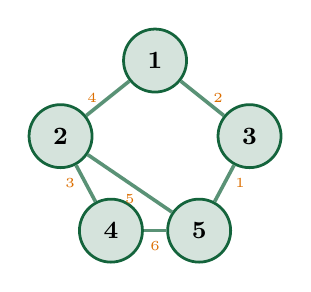
\begin{tikzpicture}[scale=0.80]
        \node[vnoG](a) at (1.5,3.0){1};
        \node[vnoG](b) at (0.0,1.8){2};
        \node[vnoG](c) at (3.0,1.8){3};
        \node[vnoG](d) at (0.8,0.3){4};
        \node[vnoG](e) at (2.2,0.3){5};
        \draw[enoG](a)--(b) node[midway,left,font=\tiny,gemaOrange]{4};
        \draw[enoG](a)--(c) node[midway,right,font=\tiny,gemaOrange]{2};
        \draw[enoG](b)--(d) node[midway,left,font=\tiny,gemaOrange]{3};
        \draw[enoG](c)--(e) node[midway,right,font=\tiny,gemaOrange]{1};
        \draw[enoG](b)--(e) node[midway,below,font=\tiny,gemaOrange]{5};
        \draw[enoG](d)--(e) node[midway,below,font=\tiny,gemaOrange]{6};
      \end{tikzpicture}
      \vspace{0.2cm}
      
\includegraphics[width=0.50\linewidth]{logo.png}
  \end{columns}
\end{frame}
}


% ─────────────────────────────────────────────────────────────
%  AGENDA
% ─────────────────────────────────────────────────────────────
\begin{frame}{Agenda}
  \begin{columns}[t]
    \column{0.47\textwidth}
      \begin{block}{Parte 1 --- Fundamentos}
        \begin{enumerate}\footnotesize
          \item Definição de grafo
          \item Terminologia essencial
          \item Tipos de grafos
          \item Lista de Adjacência
          \item Matriz de Adjacência
          \item Lista de Arestas
        \end{enumerate}
      \end{block}
    \column{0.47\textwidth}
      \begin{block}{Parte 2 --- Algoritmos}
        \begin{enumerate}\footnotesize
          \item BFS (Busca em Largura)
          \item DFS (Busca em Profundidade)
          \item Dijkstra (caminho mínimo)
          \item MST: Kruskal e Prim
          \item Fluxo Máximo (conceito)
          \item Ordenação Topológica
        \end{enumerate}
      \end{block}
  \end{columns}
  \vspace{0.2cm}
  \begin{tcolorbox}[caixaAmarelo,title={Objetivo da aula}]
    \small
    Entender grafos, \textbf{representá-los em C++} e aplicar
    \textbf{BFS, DFS e Dijkstra} em problemas de maratona.
  \end{tcolorbox}
\end{frame}

% =============================================================
%  DIVISOR PARTE 1
% =============================================================
{
\setbeamertemplate{footline}{}
\begin{frame}[noframenumbering]
  \centering\vspace{1.2cm}
  {\fontsize{38}{46}\selectfont\bfseries\color{gemaBlue} 1}\par
  \vspace{0.25cm}
  {\Large\color{graphColor}\bfseries Fundamentos de Grafos}\par
  \vspace{0.15cm}
  {\color{gray}\small Definição $\cdot$ Terminologia $\cdot$ Tipos}
\end{frame}
}

% ─────────────────────────────────────────────────────────────
%  DEFINIÇÃO DE GRAFO
% ─────────────────────────────────────────────────────────────
\begin{frame}{O que é um Grafo?}
  \begin{columns}[c]
    \column{0.48\textwidth}
      \begin{tcolorbox}[caixaGrafo,title={Definição Formal}]
        \small
        Um \textbf{grafo} $G = (V, E)$ é composto por:\\[3pt]
        $V$ = conjunto de \textbf{vértices} (nós)\\
        $E$ = conjunto de \textbf{arestas} (conexões)\\[4pt]
        Cada aresta $(u, v) \in E$ liga dois vértices.
      \end{tcolorbox}
      \vspace{0.12cm}
      \begin{tcolorbox}[caixaAzul,title={Exemplos do mundo real}]
        \begin{itemize}\footnotesize
          \item Cidades (vértices) e estradas (arestas)
          \item Páginas web e hiperlinks
          \item Amigos em uma rede social
          \item Computadores em uma rede
          \item Dependências em um projeto
        \end{itemize}
      \end{tcolorbox}
      \vspace{0.08cm}
      \begin{tcolorbox}[caixaAmarelo,title={Na OBI}]
        \footnotesize
        Grafos aparecem em: labirintos, mapas,\\
        redes de comunicação, fluxos, jogos.
      \end{tcolorbox}
    \column{0.50\textwidth}
      \centering
      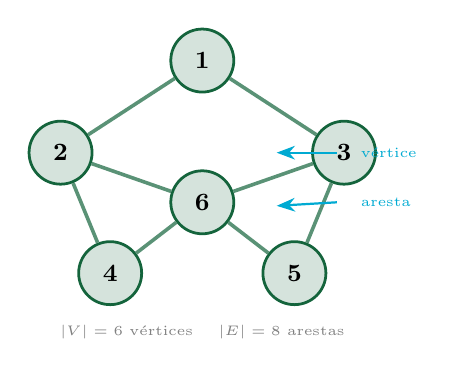
\begin{tikzpicture}[scale=0.90]
        \node[vnoG](1) at (2.5,3.5){1};
        \node[vnoG](2) at (0.5,2.2){2};
        \node[vnoG](3) at (4.5,2.2){3};
        \node[vnoG](4) at (1.2,0.5){4};
        \node[vnoG](5) at (3.8,0.5){5};
        \node[vnoG](6) at (2.5,1.5){6};
        \draw[enoG](1)--(2);
        \draw[enoG](1)--(3);
        \draw[enoG](2)--(4);
        \draw[enoG](2)--(6);
        \draw[enoG](3)--(5);
        \draw[enoG](3)--(6);
        \draw[enoG](4)--(6);
        \draw[enoG](5)--(6);
        \node[font=\tiny,gray,below] at (2.5,-0.1)
          {$|V| = 6$ vértices \quad $|E| = 8$ arestas};
        % Labels
        \node[font=\tiny,gemaCyan,right] at (4.6,2.2){vértice};
        \draw[-{Stealth},gemaCyan,line width=0.8pt](4.4,2.2)--(3.55,2.2);
        \node[font=\tiny,gemaCyan,right] at (4.6,1.5){aresta};
        \draw[-{Stealth},gemaCyan,line width=0.8pt](4.4,1.5)--(3.55,1.45);
      \end{tikzpicture}
  \end{columns}
\end{frame}

% ─────────────────────────────────────────────────────────────
%  TERMINOLOGIA
% ─────────────────────────────────────────────────────────────
\begin{frame}{Terminologia Essencial}
  \begin{columns}[t]
    \column{0.30\textwidth}
      \begin{tcolorbox}[caixaGrafo,title={Grau}]
        \footnotesize
        \textbf{Grau} de um vértice = número de arestas que incidem sobre ele.\\[4pt]
        Em grafos direcionados:\\
        \textbf{grau de entrada} (in-degree)\\
        \textbf{grau de saída} (out-degree)
      \end{tcolorbox}
      \vspace{0.08cm}
      \begin{tcolorbox}[caixaAzul,title={Caminho}]
        \footnotesize
        Sequência de vértices\\
        $v_1 \to v_2 \to \cdots \to v_k$\\
        onde cada par consecutivo é ligado por aresta.\\[3pt]
        \textbf{Comprimento} = nº arestas no caminho.
      \end{tcolorbox}
    \column{0.30\textwidth}
      \begin{tcolorbox}[caixaDfs,title={Ciclo}]
        \footnotesize
        Caminho que começa e termina no mesmo vértice.\\[4pt]
        Grafo \textbf{acíclico}: sem ciclos.\\[4pt]
        \textbf{DAG} = Directed Acyclic Graph.
      \end{tcolorbox}
      \vspace{0.08cm}
      \begin{tcolorbox}[caixaVerde,title={Conectividade}]
        \footnotesize
        Grafo \textbf{conexo}: existe caminho entre todo par de vértices.\\[4pt]
        \textbf{Componente conexa}: subgrafo maximal conexo.
      \end{tcolorbox}
    \column{0.35\textwidth}
      \centering
      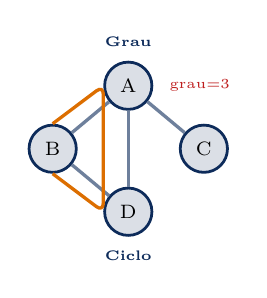
\begin{tikzpicture}[scale=0.80]
        % Grau
        \node[font=\tiny\bfseries,gemaBlue] at (1.5,4.2){Grau};
        \node[vno,minimum size=6mm,font=\scriptsize](c1) at (1.5,3.5){A};
        \node[vno,minimum size=6mm,font=\scriptsize](c2) at (0.3,2.5){B};
        \node[vno,minimum size=6mm,font=\scriptsize](c3) at (2.7,2.5){C};
        \node[vno,minimum size=6mm,font=\scriptsize](c4) at (1.5,1.5){D};
        \draw[eno](c1)--(c2); \draw[eno](c1)--(c3);
        \draw[eno](c1)--(c4); \draw[eno](c2)--(c4);
        \node[gemaRed,font=\tiny,right] at (2.0,3.5){grau=3};

        % Ciclo
        \node[font=\tiny\bfseries,gemaBlue] at (1.5,0.8){Ciclo};
        \draw[gemaOrange,very thick,rounded corners=3pt]
          (c2.south)--(c4.west)--(c1.west)--(c2.north);
      \end{tikzpicture}
  \end{columns}
\end{frame}

% ─────────────────────────────────────────────────────────────
%  TIPOS DE GRAFOS
% ─────────────────────────────────────────────────────────────
\begin{frame}{Tipos de Grafos}
  \centering
  \begin{adjustbox}{max totalsize={0.97\textwidth}{0.78\textheight},center}
  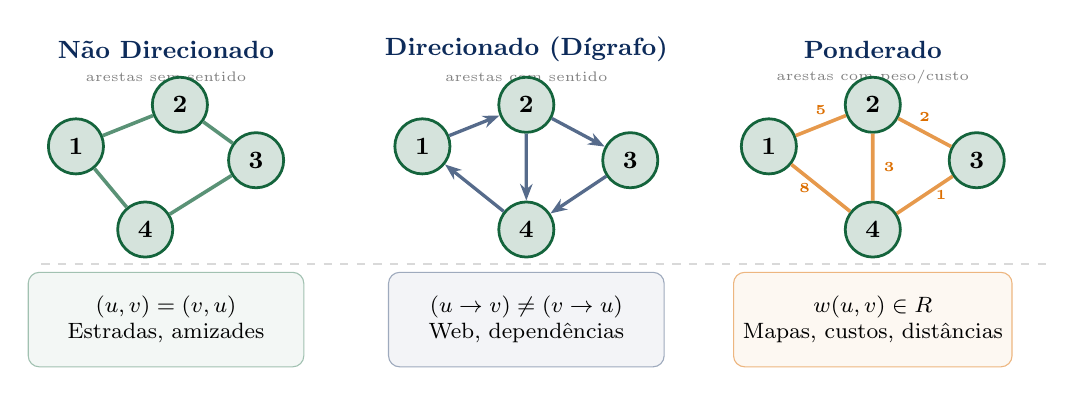
\begin{tikzpicture}[scale=0.88]

    % ── Não Direcionado ────────────────────────────────────
    \node[font=\bfseries\small,gemaBlue] at (1.8,4.6){Não Direcionado};
    \node[font=\tiny,gray] at (1.8,4.2){arestas sem sentido};
    \node[vnoG,minimum size=7mm](a1) at (0.5,3.2){1};
    \node[vnoG,minimum size=7mm](a2) at (2.0,3.8){2};
    \node[vnoG,minimum size=7mm](a3) at (3.1,3.0){3};
    \node[vnoG,minimum size=7mm](a4) at (1.5,2.0){4};
    \draw[enoG](a1)--(a2); \draw[enoG](a2)--(a3);
    \draw[enoG](a1)--(a4); \draw[enoG](a3)--(a4);

    % ── Direcionado ────────────────────────────────────────
    \node[font=\bfseries\small,gemaBlue] at (7.0,4.6){Direcionado (Dígrafo)};
    \node[font=\tiny,gray] at (7.0,4.2){arestas com sentido};
    \node[vnoG,minimum size=7mm](b1) at (5.5,3.2){1};
    \node[vnoG,minimum size=7mm](b2) at (7.0,3.8){2};
    \node[vnoG,minimum size=7mm](b3) at (8.5,3.0){3};
    \node[vnoG,minimum size=7mm](b4) at (7.0,2.0){4};
    \draw[edir](b1)--(b2); \draw[edir](b2)--(b3);
    \draw[edir](b3)--(b4); \draw[edir](b4)--(b1);
    \draw[edir](b2)--(b4);

    % ── Ponderado ──────────────────────────────────────────
    \node[font=\bfseries\small,gemaBlue] at (12.0,4.6){Ponderado};
    \node[font=\tiny,gray] at (12.0,4.2){arestas com peso/custo};
    \node[vnoG,minimum size=7mm](c1) at (10.5,3.2){1};
    \node[vnoG,minimum size=7mm](c2) at (12.0,3.8){2};
    \node[vnoG,minimum size=7mm](c3) at (13.5,3.0){3};
    \node[vnoG,minimum size=7mm](c4) at (12.0,2.0){4};
    \draw[epeso](c1)--(c2) node[midway,above,font=\tiny\bfseries,gemaOrange]{5};
    \draw[epeso](c2)--(c3) node[midway,above,font=\tiny\bfseries,gemaOrange]{2};
    \draw[epeso](c1)--(c4) node[midway,left,font=\tiny\bfseries,gemaOrange]{8};
    \draw[epeso](c3)--(c4) node[midway,right,font=\tiny\bfseries,gemaOrange]{1};
    \draw[epeso](c2)--(c4) node[midway,right,font=\tiny\bfseries,gemaOrange]{3};

    % ── Linha divisora ─────────────────────────────────────
    \draw[gray!30,dashed,line width=0.8pt](0,1.5)--(14.5,1.5);

    % ── Descrições ─────────────────────────────────────────
    \node[draw=graphColor!40,fill=graphColor!5,rounded corners=4pt,
          font=\footnotesize,align=center,minimum width=3.5cm,minimum height=1.2cm]
      at (1.8,0.7){$(u,v) = (v,u)$\\Estradas, amizades};
    \node[draw=gemaBlue!40,fill=gemaBlue!5,rounded corners=4pt,
          font=\footnotesize,align=center,minimum width=3.5cm,minimum height=1.2cm]
      at (7.0,0.7){$(u \to v) \neq (v \to u)$\\Web, dependências};
    \node[draw=gemaOrange!50,fill=gemaOrange!5,rounded corners=4pt,
          font=\footnotesize,align=center,minimum width=3.5cm,minimum height=1.2cm]
      at (12.0,0.7){$w(u,v) \in \mathbb{R}$\\Mapas, custos, distâncias};

  \end{tikzpicture}
  \end{adjustbox}
\end{frame}

% =============================================================
%  DIVISOR REPRESENTAÇÃO
% =============================================================
{
\setbeamertemplate{footline}{}
\begin{frame}[noframenumbering]
  \centering\vspace{1.2cm}
  {\fontsize{38}{46}\selectfont\bfseries\color{gemaBlue} 2}\par
  \vspace{0.25cm}
  {\Large\color{gemaBlue}\bfseries Representação de Grafos}\par
  \vspace{0.15cm}
  {\color{gray}\small Lista de Adj. $\cdot$ Matriz $\cdot$ Lista de Arestas}
\end{frame}
}

% ─────────────────────────────────────────────────────────────
%  LISTA DE ADJACÊNCIA
% ─────────────────────────────────────────────────────────────
\begin{frame}[fragile]{Lista de Adjacência --- \texttt{vector<vector<int>>}}
  \begin{columns}[t]
    \column{0.54\textwidth}
      \begin{tcolorbox}[caixaCodigo]
        \begin{lstlisting}[style=cppstyle]
#include <bits/stdc++.h>
using namespace std;

int main() {
    int N = 5, M = 6; // vertices, arestas
    vector<vector<int>> adj(N + 1);

    // Grafo nao direcionado
    // aresta (u, v)
    adj[1].push_back(2);
    adj[2].push_back(1);
    adj[1].push_back(3);
    adj[3].push_back(1);
    // ...lendo da entrada:
    for (int i = 0; i < M; i++) {
        int u, v; cin >> u >> v;
        adj[u].push_back(v);
        adj[v].push_back(u); // omite se dirigido
    }

    // Iterando vizinhos de v
    int v = 1;
    for (int u : adj[v]) {
        cout << v << " -> " << u << "\n";
    }
    return 0;
}
        \end{lstlisting}
      \end{tcolorbox}
    \column{0.44\textwidth}
      \begin{tcolorbox}[caixaGrafo,title={Visualização}]
        \centering\footnotesize
        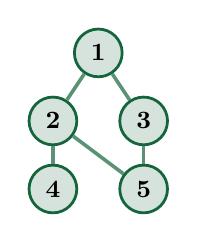
\begin{tikzpicture}[scale=0.72]
          \node[vnoG,minimum size=6mm](n1) at (0.8,2.8){1};
          \node[vnoG,minimum size=6mm](n2) at (0.0,1.6){2};
          \node[vnoG,minimum size=6mm](n3) at (1.6,1.6){3};
          \node[vnoG,minimum size=6mm](n4) at (0.0,0.4){4};
          \node[vnoG,minimum size=6mm](n5) at (1.6,0.4){5};
          \draw[enoG](n1)--(n2); \draw[enoG](n1)--(n3);
          \draw[enoG](n2)--(n4); \draw[enoG](n3)--(n5);
          \draw[enoG](n2)--(n5);
        \end{tikzpicture}
        \quad
        \begin{tabular}{r|l}
          \textbf{v} & \textbf{adj[v]}\\
          \hline
          1 & [2, 3]\\
          2 & [1, 4, 5]\\
          3 & [1, 5]\\
          4 & [2]\\
          5 & [3, 2]\\
        \end{tabular}
      \end{tcolorbox}
      \vspace{0.07cm}
      \begin{tcolorbox}[caixaVerde,title={Vantagens}]
        \footnotesize
        Espaço: \textbf{O(V + E)}\\
        Iterar vizinhos: \textbf{O(grau)}\\
        \textbf{Padrão em maratona}\\
        Funciona bem com V, E grandes
      \end{tcolorbox}
      \vspace{0.07cm}
      \begin{tcolorbox}[caixaLaranja,title={Grafo ponderado}]
        \footnotesize
        \texttt{vector<vector<pair<int,int>>>}\\
        \texttt{adj[u].push\_back(\{v, peso\});}
      \end{tcolorbox}
  \end{columns}
\end{frame}

% ─────────────────────────────────────────────────────────────
%  MATRIZ DE ADJACÊNCIA
% ─────────────────────────────────────────────────────────────
\begin{frame}[fragile]{Matriz de Adjacência --- \texttt{int adj[N][N]}}
  \begin{columns}[t]
    \column{0.50\textwidth}
      \begin{tcolorbox}[caixaCodigo]
        \begin{lstlisting}[style=cppstyle]
#include <bits/stdc++.h>
using namespace std;

const int MAXN = 1001;
int adj[MAXN][MAXN];

int main() {
    int N, M; cin >> N >> M;
    // adj[u][v] = 1 se existe aresta
    // adj[u][v] = peso se ponderado

    for (int i = 0; i < M; i++) {
        int u, v; cin >> u >> v;
        adj[u][v] = 1;
        adj[v][u] = 1; // nao dirigido
    }

    // Verificar aresta (u,v): O(1)
    if (adj[2][3]) {
        cout << "Existe aresta 2-3\n";
    }

    // Vizinhos de v: O(N)
    for (int u = 1; u <= N; u++) {
        if (adj[3][u])
            cout << "3 -> " << u << "\n";
    }
}
        \end{lstlisting}
      \end{tcolorbox}
    \column{0.48\textwidth}
      \centering
      \begin{tcolorbox}[caixaAzul,title={Matriz para o grafo}]
        \centering\footnotesize
        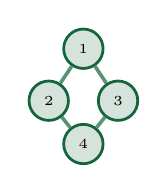
\begin{tikzpicture}[scale=0.55]
          \node[vnoG,minimum size=5mm,font=\tiny](n1) at (0.8,2.2){1};
          \node[vnoG,minimum size=5mm,font=\tiny](n2) at (0.0,1.0){2};
          \node[vnoG,minimum size=5mm,font=\tiny](n3) at (1.6,1.0){3};
          \node[vnoG,minimum size=5mm,font=\tiny](n4) at (0.8,0.0){4};
          \draw[enoG](n1)--(n2); \draw[enoG](n1)--(n3);
          \draw[enoG](n2)--(n4); \draw[enoG](n3)--(n4);
        \end{tikzpicture}
        \quad
        $\begin{pmatrix}
          0 & 1 & 1 & 0\\
          1 & 0 & 0 & 1\\
          1 & 0 & 0 & 1\\
          0 & 1 & 1 & 0
        \end{pmatrix}$
      \end{tcolorbox}
      \vspace{0.07cm}
      \begin{tcolorbox}[caixaVerde,title={Quando usar}]
        \footnotesize
        Verificar aresta em \textbf{O(1)}\\
        Grafos \textbf{densos} ($E \approx V^2$)\\
        $N \leq 1000$ (cabe na memória)
      \end{tcolorbox}
      \vspace{0.07cm}
      \begin{tcolorbox}[caixaVermelho,title={Quando NÃO usar}]
        \footnotesize
        $N > 1000$: memória explode!\\
        $N = 10^5$: $10^{10}$ bytes \texttimes\\[2pt]
        Grafos \textbf{esparsos}: desperdício\\
        \textbf{Prefira lista de adjacência}
      \end{tcolorbox}
  \end{columns}
\end{frame}

% ─────────────────────────────────────────────────────────────
%  LISTA DE ARESTAS
% ─────────────────────────────────────────────────────────────
\begin{frame}[fragile]{Lista de Arestas --- \texttt{vector<pair<int,int>>}}
  \begin{columns}[t]
    \column{0.52\textwidth}
      \begin{tcolorbox}[caixaCodigo]
        \begin{lstlisting}[style=cppstyle]
#include <bits/stdc++.h>
using namespace std;

struct Aresta {
    int u, v, peso;
    // Para Kruskal: ordena por peso
    bool operator<(const Aresta& o) const {
        return peso < o.peso;
    }
};

int main() {
    int M; cin >> M;
    vector<Aresta> arestas(M);

    for (auto& [u, v, w] : arestas) {
        cin >> u >> v >> w;
    }

    // Ordenar por peso (para Kruskal)
    sort(arestas.begin(), arestas.end());

    for (auto& [u, v, w] : arestas) {
        cout << u << "-" << v
             << " w=" << w << "\n";
    }
}
        \end{lstlisting}
      \end{tcolorbox}
    \column{0.46\textwidth}
      \begin{tcolorbox}[caixaGrafo,title={Exemplo}]
        \footnotesize
        Grafo com 4 vértices:\\[3pt]
        \begin{tabular}{ccc}
          \textbf{u} & \textbf{v} & \textbf{peso}\\
          \hline
          1 & 2 & 4\\
          1 & 3 & 2\\
          2 & 3 & 5\\
          3 & 4 & 1\\
        \end{tabular}\\[5pt]
        Após sort: 3-4(1), 1-3(2), 1-2(4), 2-3(5)
      \end{tcolorbox}
      \vspace{0.07cm}
      \begin{tcolorbox}[caixaVerde,title={Quando usar}]
        \footnotesize
        Algoritmo de \textbf{Kruskal} (MST)\\
        Precisar \textbf{ordenar arestas}\\
        Algoritmos de fluxo simples
      \end{tcolorbox}
      \vspace{0.07cm}
      \begin{tcolorbox}[caixaVermelho,title={Desvantagem}]
        \footnotesize
        Achar vizinhos de $v$: \textbf{O(E)}\\
        Não adequado para BFS/DFS/Dijkstra\\
        Use lista de adjacência nestes casos
      \end{tcolorbox}
  \end{columns}
\end{frame}

% ─────────────────────────────────────────────────────────────
%  TABELA COMPARATIVA
% ─────────────────────────────────────────────────────────────
\begin{frame}{Comparação das Representações}
  \begin{tcolorbox}[caixaAzul,title={Tabela Comparativa}]
    \centering\footnotesize
    \begin{tabular}{lcccl}
      \toprule
      \textbf{Representação} & \textbf{Espaço} & \textbf{Aresta(u,v)?} &
      \textbf{Vizinhos(v)} & \textbf{Melhor uso}\\
      \midrule
      Lista de Adj.    & O(V+E)   & O(grau)  & O(grau)  & BFS, DFS, Dijkstra\\
      Matriz de Adj.   & O(V$^2$) & O(1)     & O(V)     & Grafos densos, $N \le 1000$\\
      Lista de Arestas & O(E)     & O(E)     & O(E)     & Kruskal, sort por peso\\
      \bottomrule
    \end{tabular}
  \end{tcolorbox}
  \vspace{0.12cm}
  \begin{columns}[t]
    \column{0.32\textwidth}
      \begin{tcolorbox}[caixaGrafo,title={Lista de Adjacência}]
        \footnotesize
        \textbf{Use sempre por padrão}\\[3pt]
        $N \le 2 \times 10^5$\\
        $E \le 5 \times 10^5$\\[3pt]
        \texttt{vector<vector<int>>}\\
        \texttt{vector<vector<pii>>}
      \end{tcolorbox}
    \column{0.32\textwidth}
      \begin{tcolorbox}[caixaAzul,title={Matriz de Adjacência}]
        \footnotesize
        \textbf{Grafos pequenos e densos}\\[3pt]
        $N \le 500$ (seguro)\\
        $N \le 1000$ (checar memória)\\[3pt]
        Fácil de programar\\
        Floyd-Warshall usa matriz
      \end{tcolorbox}
    \column{0.32\textwidth}
      \begin{tcolorbox}[caixaLaranja,title={Lista de Arestas}]
        \footnotesize
        \textbf{Kruskal e algoritmos}\\
        \textbf{que ordenam arestas}\\[3pt]
        Simples de ler da entrada\\[3pt]
        \texttt{vector<Aresta>}\\
        \texttt{sort(edges.begin(), ...)}
      \end{tcolorbox}
  \end{columns}
  \vspace{0.10cm}
  \begin{tcolorbox}[caixaAmarelo,title={Regra de ouro}]
    \footnotesize
    \textbf{Padrão de maratona:} Liste de adjacência para quase tudo.
    Só mude quando o algoritmo exigir (Kruskal $\to$ lista de arestas,
    Floyd-Warshall $\to$ matriz).
  \end{tcolorbox}
\end{frame}

% =============================================================
%  DIVISOR BFS
% =============================================================
{
\setbeamertemplate{footline}{}
\begin{frame}[noframenumbering]
  \centering\vspace{1.2cm}
  {\fontsize{38}{46}\selectfont\bfseries\color{gemaBlue} 3}\par
  \vspace{0.25cm}
  {\Large\color{queueColor}\bfseries BFS --- Busca em Largura}\par
  \vspace{0.15cm}
  {\color{gray}\small Nível por nível $\cdot$ Menor caminho sem peso $\cdot$ Grade}
\end{frame}
}

% ─────────────────────────────────────────────────────────────
%  BFS — CONCEITO VISUAL
% ─────────────────────────────────────────────────────────────
\begin{frame}{BFS --- Exploração Nível por Nível}
  \centering
  \begin{adjustbox}{max totalsize={0.98\textwidth}{0.80\textheight},center}
  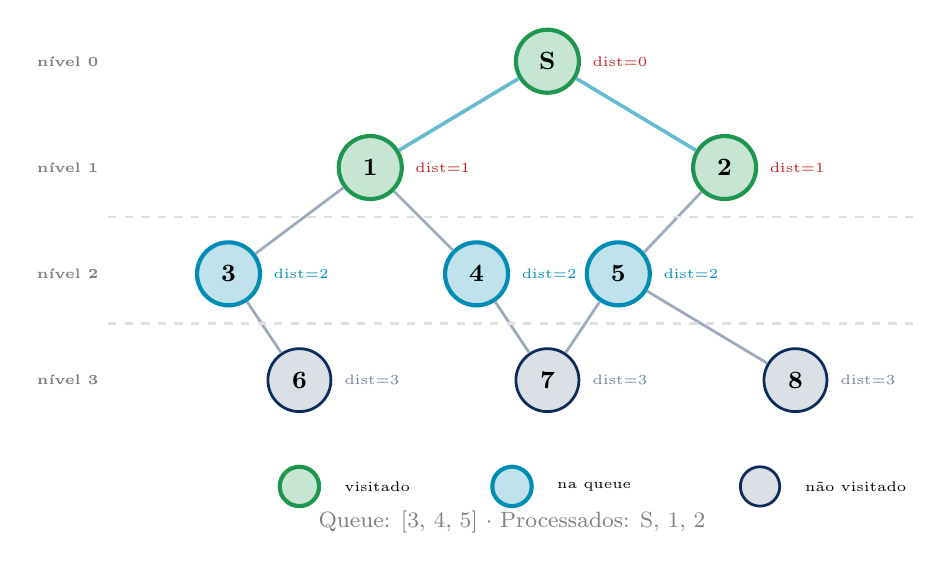
\begin{tikzpicture}[scale=0.90]

    % Nós
    \node[vnoVis](s)  at (6.0,5.5){S};
    \node[vnoVis](n1) at (3.5,4.0){1};
    \node[vnoVis](n2) at (8.5,4.0){2};
    \node[vnoBFS](n3) at (1.5,2.5){3};
    \node[vnoBFS](n4) at (5.0,2.5){4};
    \node[vnoBFS](n5) at (7.0,2.5){5};
    \node[vno]   (n6) at (2.5,1.0){6};
    \node[vno]   (n7) at (6.0,1.0){7};
    \node[vno]   (n8) at (9.5,1.0){8};

    % Arestas
    \draw[queueColor!60,line width=1.3pt](s)--(n1);
    \draw[queueColor!60,line width=1.3pt](s)--(n2);
    \draw[gemaBlue!40,line width=1.0pt](n1)--(n3);
    \draw[gemaBlue!40,line width=1.0pt](n1)--(n4);
    \draw[gemaBlue!40,line width=1.0pt](n2)--(n5);
    \draw[gemaBlue!40,line width=1.0pt](n3)--(n6);
    \draw[gemaBlue!40,line width=1.0pt](n4)--(n7);
    \draw[gemaBlue!40,line width=1.0pt](n5)--(n7);
    \draw[gemaBlue!40,line width=1.0pt](n5)--(n8);

    % Linhas de nível
    \draw[gray!25,dashed,line width=0.8pt](-0.2,3.3)--(11.2,3.3);
    \draw[gray!25,dashed,line width=0.8pt](-0.2,1.8)--(11.2,1.8);

    % Labels de nível
    \node[font=\tiny\bfseries,gray,left] at (-0.2,5.5){nível 0};
    \node[font=\tiny\bfseries,gray,left] at (-0.2,4.0){nível 1};
    \node[font=\tiny\bfseries,gray,left] at (-0.2,2.5){nível 2};
    \node[font=\tiny\bfseries,gray,left] at (-0.2,1.0){nível 3};

    % Distâncias
    \node[font=\tiny,gemaRed,right] at (6.5,5.5){dist=0};
    \node[font=\tiny,gemaRed,right] at (4.0,4.0){dist=1};
    \node[font=\tiny,gemaRed,right] at (9.0,4.0){dist=1};
    \node[font=\tiny,queueColor,right] at (2.0,2.5){dist=2};
    \node[font=\tiny,queueColor,right] at (5.5,2.5){dist=2};
    \node[font=\tiny,queueColor,right] at (7.5,2.5){dist=2};
    \node[font=\tiny,gemaBlue!60,right] at (3.0,1.0){dist=3};
    \node[font=\tiny,gemaBlue!60,right] at (6.5,1.0){dist=3};
    \node[font=\tiny,gemaBlue!60,right] at (10.0,1.0){dist=3};

    % Legenda
    \node[vnoVis,minimum size=5mm] at (2.5,-0.5){};
    \node[font=\tiny,right] at (3.0,-0.5){visitado};
    \node[vnoBFS,minimum size=5mm] at (5.5,-0.5){};
    \node[font=\tiny,right] at (6.0,-0.5){na queue};
    \node[vno,minimum size=5mm] at (9.0,-0.5){};
    \node[font=\tiny,right] at (9.5,-0.5){não visitado};

    \node[font=\footnotesize,gray] at (5.5,-1.0)
      {Queue: [3, 4, 5] $\cdot$ Processados: S, 1, 2};
  \end{tikzpicture}
  \end{adjustbox}
\end{frame}

% ─────────────────────────────────────────────────────────────
%  BFS — CÓDIGO COMPLETO
% ─────────────────────────────────────────────────────────────
\begin{frame}[fragile,shrink=3]{BFS --- Código Completo em C++}
  \begin{columns}[t]
    \column{0.56\textwidth}
      \begin{tcolorbox}[caixaCodigo]
        \begin{lstlisting}[style=cppsmall]
#include <bits/stdc++.h>
using namespace std;

// BFS em grafo geral
// Retorna vetor de distancias a partir de 'inicio'
vector<int> bfs(int inicio, int N,
    vector<vector<int>>& adj) {

    vector<bool> vis(N+1, false);
    vector<int>  dist(N+1, -1);
    queue<int> q;

    vis[inicio]  = true;
    dist[inicio] = 0;
    q.push(inicio);

    while (!q.empty()) {
        int v = q.front(); q.pop();

        for (int u : adj[v]) {
            if (!vis[u]) {
                vis[u]  = true;
                dist[u] = dist[v] + 1;
                q.push(u);
            }
        }
    }
    return dist;
}

int main() {
    int N, M; cin >> N >> M;
    vector<vector<int>> adj(N+1);
    for (int i = 0; i < M; i++) {
        int u, v; cin >> u >> v;
        adj[u].push_back(v);
        adj[v].push_back(u);
    }
    auto dist = bfs(1, N, adj);
    for (int i = 1; i <= N; i++)
        cout << "dist[" << i << "] = "
             << dist[i] << "\n";
}
        \end{lstlisting}
      \end{tcolorbox}
    \column{0.42\textwidth}
      \begin{tcolorbox}[caixaAzul,title={Invariante da BFS}]
        \footnotesize
        A queue sempre contém nós\\
        de \textbf{no máximo 2 níveis} distintos.\\[4pt]
        Nós do nível $k$ são processados\\
        \textbf{antes} de qualquer nó do nível $k+1$.\\[4pt]
        Isso garante \textbf{menor caminho}.
      \end{tcolorbox}
      \vspace{0.08cm}
      \begin{tcolorbox}[caixaVerde,title={Complexidade}]
        \footnotesize
        \textbf{Tempo:} O(V + E)\\
        Cada vértice entra/sai 1x\\
        Cada aresta é verificada 1x\\[3pt]
        \textbf{Espaço:} O(V)\\
        Vetores vis, dist e queue
      \end{tcolorbox}
      \vspace{0.08cm}
      \begin{tcolorbox}[caixaAmarelo,title={Aplicações}]
        \footnotesize
        Menor caminho sem pesos\\
        Labirintos e grades (grid)\\
        Componentes conexas\\
        Verificar bipartição\\
        Propagação por ``ondas''
      \end{tcolorbox}
      \vspace{0.08cm}
      \begin{tcolorbox}[caixaVermelho,title={Atenção}]
        \footnotesize
        BFS \textbf{não} encontra menor\\
        caminho em grafos com pesos.\\
        Para pesos $\to$ \textbf{Dijkstra}!
      \end{tcolorbox}
  \end{columns}
\end{frame}

% ─────────────────────────────────────────────────────────────
%  BFS EM GRADE (GRID)
% ─────────────────────────────────────────────────────────────
\begin{frame}[fragile,shrink=3]{BFS em Grade (Grid) --- Labirinto}
  \begin{columns}[t]
    \column{0.54\textwidth}
      \begin{tcolorbox}[caixaCodigo]
        \begin{lstlisting}[style=cppsmall]
#include <bits/stdc++.h>
using namespace std;

int N, M;
char grid[305][305];
int  dist[305][305];
// 4 direcoes: cima, baixo, esq, dir
int dx[] = {-1, 1,  0, 0};
int dy[] = { 0, 0, -1, 1};

bool valido(int x, int y) {
    return x>=0 && x<N && y>=0 && y<M
           && grid[x][y] != '#'
           && dist[x][y] == -1;
}

int bfsGrid(int sx, int sy,
            int ex, int ey) {
    memset(dist, -1, sizeof(dist));
    queue<pair<int,int>> q;
    dist[sx][sy] = 0;
    q.push({sx, sy});

    while (!q.empty()) {
        auto [x, y] = q.front(); q.pop();
        if (x == ex && y == ey)
            return dist[x][y];
        for (int d = 0; d < 4; d++) {
            int nx = x + dx[d];
            int ny = y + dy[d];
            if (valido(nx, ny)) {
                dist[nx][ny] = dist[x][y]+1;
                q.push({nx, ny});
            }
        }
    }
    return -1; // sem caminho
}
        \end{lstlisting}
      \end{tcolorbox}
    \column{0.44\textwidth}
      \centering
      \begin{tcolorbox}[caixaAzul,title={Grade exemplo}]
        \centering\footnotesize
        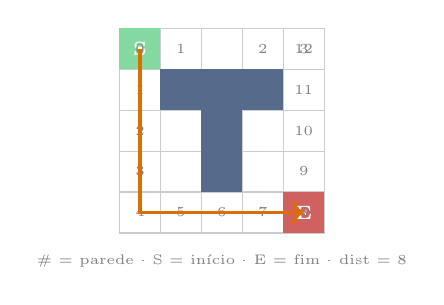
\begin{tikzpicture}[scale=0.52]
          % Grade 5x5
          \foreach \i in {0,...,4}{
            \foreach \j in {0,...,4}{
              \draw[gray!40](\j,\i) rectangle (\j+1,\i+1);
            }
          }
          % Paredes
          \foreach \pos in {(1,3),(2,3),(3,3),(2,2),(2,1)}{
            \fill[gemaBlue!70]\pos rectangle ++(1,1);
          }
          % Inicio e fim
          \fill[codeGreen!70](0,4) rectangle ++(1,1);
          \node[white,font=\bfseries\scriptsize] at (0.5,4.5){S};
          \fill[gemaRed!70](4,0) rectangle ++(1,1);
          \node[white,font=\bfseries\scriptsize] at (4.5,0.5){E};
          % Distancias
          \foreach \x/\y/\d in {
            0/4/0, 0/3/1, 0/2/2, 0/1/3, 0/0/4,
            1/4/1,
            1/0/5, 2/0/6, 3/0/7, 4/0/8,
            4/1/9, 4/2/10, 4/3/11, 4/4/12,
            3/4/2, 4/4/3
          }{
            \node[font=\fontsize{4}{4}\selectfont,gray] at (\x+0.5,\y+0.5){\d};
          }
          % Caminho ótimo (setas)
          \draw[gemaOrange,very thick,->]
            (0.5,4.5)--(0.5,3.5)--(0.5,2.5)--(0.5,1.5)--(0.5,0.5)
            --(1.5,0.5)--(2.5,0.5)--(3.5,0.5)--(4.5,0.5);
          \node[font=\tiny,gray,below] at (2.5,-0.3)
            {\# = parede · S = início · E = fim · dist = 8};
        \end{tikzpicture}
      \end{tcolorbox}
      \vspace{0.07cm}
      \begin{tcolorbox}[caixaVerde,title={Padrão Grid BFS}]
        \footnotesize
        \textbf{4-vizinhos:} dx/dy arrays\\
        \textbf{8-vizinhos:} incluir diagonais\\[3pt]
        Checar: dentro dos limites\\
        + não é parede + não visitado
      \end{tcolorbox}
      \vspace{0.07cm}
      \begin{tcolorbox}[caixaAmarelo,title={Complexidade Grid}]
        \footnotesize
        $N \times M$ células\\
        \textbf{O(N $\times$ M)}
      \end{tcolorbox}
  \end{columns}
\end{frame}

% =============================================================
%  DIVISOR DFS
% =============================================================
{
\setbeamertemplate{footline}{}
\begin{frame}[noframenumbering]
  \centering\vspace{1.2cm}
  {\fontsize{38}{46}\selectfont\bfseries\color{gemaBlue} 4}\par
  \vspace{0.25cm}
  {\Large\color{dfsColor}\bfseries DFS --- Busca em Profundidade}\par
  \vspace{0.15cm}
  {\color{gray}\small Recursivo $\cdot$ Componentes Conexas $\cdot$ Ciclos}
\end{frame}
}

% ─────────────────────────────────────────────────────────────
%  DFS — CONCEITO VISUAL
% ─────────────────────────────────────────────────────────────
\begin{frame}{DFS --- Exploração em Profundidade}
  \centering
  \begin{adjustbox}{max totalsize={0.98\textwidth}{0.82\textheight},center}
  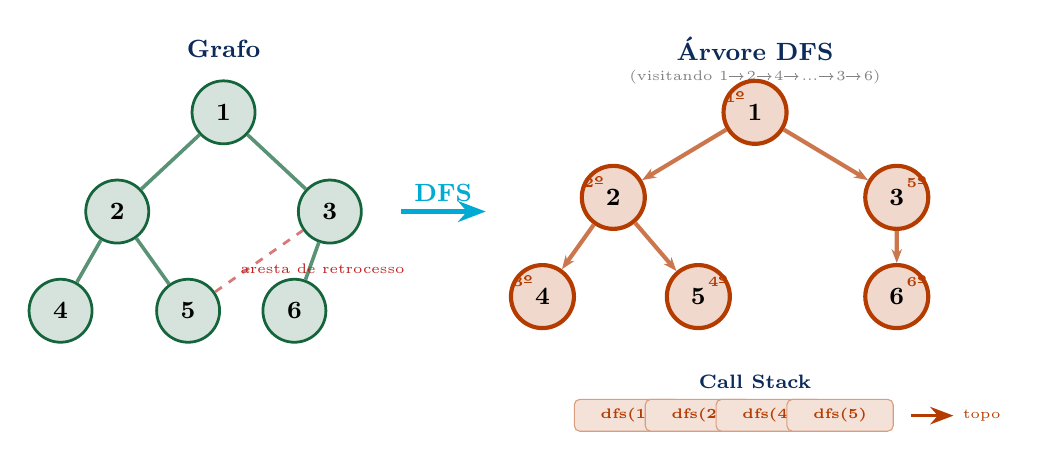
\begin{tikzpicture}[scale=0.90]

    % Grafo original (esquerda)
    \node[font=\bfseries\small,gemaBlue] at (2.5,5.5){Grafo};
    \node[vnoG](g1) at (2.5,4.6){1};
    \node[vnoG](g2) at (1.0,3.2){2};
    \node[vnoG](g3) at (4.0,3.2){3};
    \node[vnoG](g4) at (0.2,1.8){4};
    \node[vnoG](g5) at (2.0,1.8){5};
    \node[vnoG](g6) at (3.5,1.8){6};
    \draw[enoG](g1)--(g2); \draw[enoG](g1)--(g3);
    \draw[enoG](g2)--(g4); \draw[enoG](g2)--(g5);
    \draw[enoG](g3)--(g6);
    % Aresta de retrocesso (ciclo)
    \draw[gemaRed!60,dashed,line width=1pt](g5)--(g3);
    \node[font=\tiny,gemaRed,right] at (2.6,2.4){aresta de retrocesso};

    % Seta
    \draw[-{Stealth[length=10pt]},gemaCyan,line width=2pt](5.0,3.2)--(6.2,3.2);
    \node[above,gemaCyan,font=\bfseries\small] at (5.6,3.2){DFS};

    % Árvore DFS (direita)
    \node[font=\bfseries\small,gemaBlue] at (10.0,5.5){Árvore DFS};
    \node[font=\tiny,gray] at (10.0,5.1){(visitando 1→2→4→...→3→6)};
    \node[vnoDFS](d1) at (10.0,4.6){1};
    \node[vnoDFS](d2) at (8.0,3.4){2};
    \node[vnoDFS](d3) at (12.0,3.4){3};
    \node[vnoDFS](d4) at (7.0,2.0){4};
    \node[vnoDFS](d5) at (9.2,2.0){5};
    \node[vnoDFS](d6) at (12.0,2.0){6};
    % Arestas da árvore
    \draw[dfsColor!70,line width=1.5pt,-{Stealth[length=5pt]}]
      (d1)--(d2); \draw[dfsColor!70,line width=1.5pt,-{Stealth[length=5pt]}](d1)--(d3);
    \draw[dfsColor!70,line width=1.5pt,-{Stealth[length=5pt]}]
      (d2)--(d4); \draw[dfsColor!70,line width=1.5pt,-{Stealth[length=5pt]}](d2)--(d5);
    \draw[dfsColor!70,line width=1.5pt,-{Stealth[length=5pt]}](d3)--(d6);
    % Ordem de visita
    \node[dfsColor,font=\tiny\bfseries,above left] at (d1){1º};
    \node[dfsColor,font=\tiny\bfseries,above left] at (d2){2º};
    \node[dfsColor,font=\tiny\bfseries,above left] at (d4){3º};
    \node[dfsColor,font=\tiny\bfseries,above right] at (d5){4º};
    \node[dfsColor,font=\tiny\bfseries,above right] at (d3){5º};
    \node[dfsColor,font=\tiny\bfseries,above right] at (d6){6º};

    % Callstack visual
    \node[font=\bfseries\scriptsize,gemaBlue] at (10.0,0.8){Call Stack};
    \foreach \lab/\x in {dfs(1)/8.2, dfs(2)/9.2, dfs(4)/10.2, dfs(5)/11.2}{
      \draw[fill=dfsColor!15,draw=dfsColor!50,rounded corners=2pt]
        (\x-0.75,0.1) rectangle (\x+0.75,0.55)
        node[midway,font=\tiny\bfseries,dfsColor]{\lab};
    }
    \draw[-{Stealth},dfsColor,line width=1.2pt](12.2,0.32)--(12.8,0.32);
    \node[right,dfsColor,font=\tiny] at (12.8,0.32){topo};

  \end{tikzpicture}
  \end{adjustbox}
\end{frame}

% ─────────────────────────────────────────────────────────────
%  DFS — CÓDIGO
% ─────────────────────────────────────────────────────────────
\begin{frame}[fragile,shrink=3]{DFS --- Código Recursivo e Iterativo}
  \begin{columns}[t]
    \column{0.50\textwidth}
      \begin{tcolorbox}[caixaCodigo,title={\small Versão Recursiva (padrão)}]
        \begin{lstlisting}[style=cppsmall]
#include <bits/stdc++.h>
using namespace std;

vector<vector<int>> adj;
vector<bool> vis;

void dfs(int v) {
    vis[v] = true;
    cout << "visitei: " << v << "\n";

    for (int u : adj[v]) {
        if (!vis[u]) {
            dfs(u); // aprofunda
        }
    }
    // volta = pos-ordem
}

// Contar componentes conexas
int contarComponentes(int N) {
    vis.assign(N+1, false);
    int comp = 0;
    for (int v = 1; v <= N; v++) {
        if (!vis[v]) {
            dfs(v);
            comp++;
        }
    }
    return comp;
}
        \end{lstlisting}
      \end{tcolorbox}
    \column{0.48\textwidth}
      \begin{tcolorbox}[caixaCodigo,title={\small Versão Iterativa (com Stack)}]
        \begin{lstlisting}[style=cppsmall]
void dfsIterativo(int inicio, int N,
    vector<vector<int>>& adj) {

    vector<bool> vis(N+1, false);
    stack<int> st;

    st.push(inicio);
    while (!st.empty()) {
        int v = st.top(); st.pop();
        if (vis[v]) continue;
        vis[v] = true;
        cout << "visitei: " << v << "\n";
        // Push em ordem reversa para
        // manter mesma ordem da recursiva
        for (int i = adj[v].size()-1;
             i >= 0; i--) {
            int u = adj[v][i];
            if (!vis[u]) st.push(u);
        }
    }
}
        \end{lstlisting}
      \end{tcolorbox}
      \begin{tcolorbox}[caixaAmarelo,title={Recursiva vs Iterativa}]
        \footnotesize
        \textbf{Recursiva:} mais simples, \\
        risco de stack overflow para $N > 10^5$.\\[3pt]
        \textbf{Iterativa:} segura para $N$ grande,\\
        um pouco mais verbosa.
      \end{tcolorbox}
  \end{columns}
\end{frame}

% ─────────────────────────────────────────────────────────────
%  DFS — APLICAÇÕES
% ─────────────────────────────────────────────────────────────
\begin{frame}{DFS --- Aplicações Clássicas}
  \begin{columns}[t]
    \column{0.48\textwidth}
      \begin{tcolorbox}[caixaDfs,title={Componentes Conexas}]
        \footnotesize
        Execute DFS de cada vértice\\
        não visitado. Cada chamada\\
        nova = nova componente.\\[4pt]
        \centering
        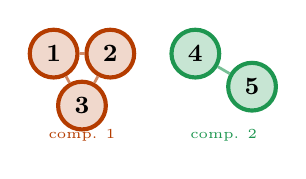
\begin{tikzpicture}[scale=0.60]
          \node[vnoDFS,minimum size=6mm](a) at (0,1.5){1};
          \node[vnoDFS,minimum size=6mm](b) at (1.2,1.5){2};
          \node[vnoDFS,minimum size=6mm](c) at (0.6,0.4){3};
          \draw[dfsColor!60,line width=1pt](a)--(b)(a)--(c)(b)--(c);
          \node[vnoVis,minimum size=6mm](d) at (3.0,1.5){4};
          \node[vnoVis,minimum size=6mm](e) at (4.2,0.8){5};
          \draw[nodeGreen!60,line width=1pt](d)--(e);
          \node[font=\tiny,dfsColor,below] at (0.6,0.1){comp. 1};
          \node[font=\tiny,nodeGreen,below] at (3.6,0.1){comp. 2};
        \end{tikzpicture}
      \end{tcolorbox}
      \vspace{0.07cm}
      \begin{tcolorbox}[caixaVerde,title={Detecção de Ciclo}]
        \footnotesize
        Grafo não dir.: ciclo existe se\\
        achamos um vizinho já visitado\\
        que \textbf{não é o pai} do nó atual.\\[3pt]
        \begin{tabular}{ll}
          \texttt{dfs(v, pai)} & $\leftarrow$ passa o pai\\
          \texttt{se vis[u] \&\&} & \\
          \texttt{u != pai:} & ciclo!
        \end{tabular}
      \end{tcolorbox}
    \column{0.48\textwidth}
      \begin{tcolorbox}[caixaAzul,title={Complexidade DFS}]
        \footnotesize
        \textbf{Tempo:} O(V + E)\\
        Cada vértice visitado 1 vez\\
        Cada aresta verificada 1-2 vezes\\[3pt]
        \textbf{Espaço:} O(V)\\
        Pilha de recursão + vis
      \end{tcolorbox}
      \vspace{0.07cm}
      \begin{tcolorbox}[caixaLaranja,title={DFS vs BFS}]
        \centering\footnotesize
        \begin{tabular}{lll}
          \toprule
          & \textbf{BFS} & \textbf{DFS}\\
          \midrule
          Estrutura & Queue & Stack\\
          Ordem & nível & profundidade\\
          Menor cam. & \textbf{sim} & não\\
          Ciclo & sim & \textbf{sim}\\
          Comp. conexas & sim & sim\\
          Topo-sort & não & \textbf{sim}\\
          Mem. pior & O(V) & O(V)\\
          \bottomrule
        \end{tabular}
      \end{tcolorbox}
      \vspace{0.07cm}
      \begin{tcolorbox}[caixaAmarelo,title={Pergunta mágica}]
        \footnotesize
        \textbf{Menor caminho?} $\to$ BFS\\
        \textbf{Explorar tudo?} $\to$ DFS\\
        \textbf{Ciclo / componentes?} $\to$ DFS
      \end{tcolorbox}
  \end{columns}
\end{frame}

% =============================================================
%  DIVISOR DIJKSTRA
% =============================================================
{
\setbeamertemplate{footline}{}
\begin{frame}[noframenumbering]
  \centering\vspace{1.2cm}
  {\fontsize{38}{46}\selectfont\bfseries\color{gemaBlue} 5}\par
  \vspace{0.25cm}
  {\Large\color{pqColor}\bfseries Dijkstra}\par
  \vspace{0.15cm}
  {\color{gray}\small Menor caminho com pesos $\cdot$ Priority Queue $\cdot$ O((V+E)log V)}
\end{frame}
}

% ─────────────────────────────────────────────────────────────
%  DIJKSTRA — POR QUE BFS NÃO BASTA
% ─────────────────────────────────────────────────────────────
\begin{frame}{Por que BFS não funciona com pesos?}
  \centering
  \begin{adjustbox}{max totalsize={0.98\textwidth}{0.78\textheight},center}
  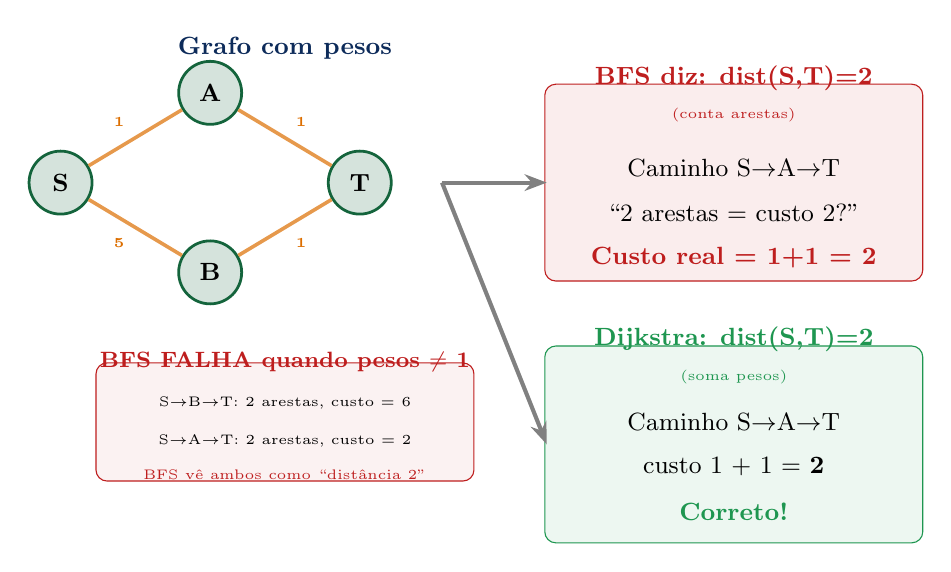
\begin{tikzpicture}[scale=0.95]

    % Grafo com pesos
    \node[font=\bfseries\small,gemaBlue] at (3.5,4.8){Grafo com pesos};

    \node[vnoG](s)  at (0.5,3.0){S};
    \node[vnoG](a)  at (2.5,4.2){A};
    \node[vnoG](b)  at (2.5,1.8){B};
    \node[vnoG](t)  at (4.5,3.0){T};

    \draw[epeso](s)--(a) node[midway,above left,font=\bfseries\tiny,gemaOrange]{1};
    \draw[epeso](s)--(b) node[midway,below left,font=\bfseries\tiny,gemaOrange]{5};
    \draw[epeso](a)--(t) node[midway,above right,font=\bfseries\tiny,gemaOrange]{1};
    \draw[epeso](b)--(t) node[midway,below right,font=\bfseries\tiny,gemaOrange]{1};

    % BFS result (errado)
    \node[draw=gemaRed,fill=gemaRed!8,rounded corners=4pt,
          minimum width=4.8cm,minimum height=2.5cm] at (9.5,3.0){};
    \node[font=\bfseries\small,gemaRed] at (9.5,4.4){BFS diz: dist(S,T)=2};
    \node[font=\tiny,gemaRed] at (9.5,3.9){(conta arestas)};
    \node[font=\small] at (9.5,3.2){Caminho S$\to$A$\to$T};
    \node[font=\small] at (9.5,2.6){``2 arestas = custo 2?''};
    \node[font=\small,gemaRed] at (9.5,2.0){\textbf{Custo real = 1+1 = 2}};

    % Dijkstra result (certo)
    \node[draw=nodeGreen,fill=nodeGreen!8,rounded corners=4pt,
          minimum width=4.8cm,minimum height=2.5cm] at (9.5,-0.5){};
    \node[font=\bfseries\small,nodeGreen] at (9.5,0.9){Dijkstra: dist(S,T)=2};
    \node[font=\tiny,nodeGreen] at (9.5,0.4){(soma pesos)};
    \node[font=\small] at (9.5,-0.2){Caminho S$\to$A$\to$T};
    \node[font=\small] at (9.5,-0.8){custo 1 + 1 = \textbf{2}};
    \node[font=\small,nodeGreen] at (9.5,-1.4){\textbf{Correto!}};

    % BFS falha real
    \node[draw=gemaRed,fill=gemaRed!6,rounded corners=4pt,
          minimum width=4.8cm,minimum height=1.5cm] at (3.5,-0.2){};
    \node[font=\bfseries\footnotesize,gemaRed] at (3.5,0.6){BFS FALHA quando pesos $\neq$ 1};
    \node[font=\tiny] at (3.5,0.05){S$\to$B$\to$T: 2 arestas, custo = 6};
    \node[font=\tiny] at (3.5,-0.45){S$\to$A$\to$T: 2 arestas, custo = 2};
    \node[font=\tiny,gemaRed] at (3.5,-0.90){BFS vê ambos como ``distância 2''};

    \draw[-{Stealth[length=8pt]},gray,line width=1.5pt](5.6,3.0)--(7.0,3.0);
    \draw[-{Stealth[length=8pt]},gray,line width=1.5pt](5.6,3.0)--(7.0,-0.5);

  \end{tikzpicture}
  \end{adjustbox}
\end{frame}

% ─────────────────────────────────────────────────────────────
%  DIJKSTRA — ALGORITMO (PASSO A PASSO)
% ─────────────────────────────────────────────────────────────
\begin{frame}{Dijkstra --- Ideia do Algoritmo}
  \begin{columns}[c]
    \column{0.47\textwidth}
      \begin{tcolorbox}[caixaRoxa,title={Algoritmo}]
        \footnotesize
        \begin{enumerate}
          \item Inicializa \texttt{dist[s]=0}, \texttt{dist[v]=$\infty$}
          \item Insere \texttt{(0, s)} na priority queue (min-heap)
          \item Enquanto PQ não vazia:
          \begin{itemize}\scriptsize
            \item Extrai \texttt{(d, v)} = menor distância
            \item Se \texttt{d > dist[v]}: ignora (desatualizado)
            \item Para cada vizinho \texttt{(u, peso)}:
            \item Se \texttt{dist[v]+peso < dist[u]}:\\
              $\quad$ \texttt{dist[u] = dist[v]+peso}\\
              $\quad$ insere \texttt{(dist[u], u)} na PQ
          \end{itemize}
        \end{enumerate}
      \end{tcolorbox}
      \vspace{0.08cm}
      \begin{tcolorbox}[caixaAmarelo,title={Relaxamento}]
        \footnotesize
        Cada vez que encontramos um caminho\\
        mais curto para \texttt{u} passando por \texttt{v},\\
        \textbf{relaxamos} a aresta \texttt{(v,u)}.\\[3pt]
        \texttt{dist[u] = min(dist[u], dist[v]+w)}
      \end{tcolorbox}
    \column{0.51\textwidth}
      \centering
      \begin{tcolorbox}[caixaAzul,title={Simulação passo a passo}]
        \centering\footnotesize
        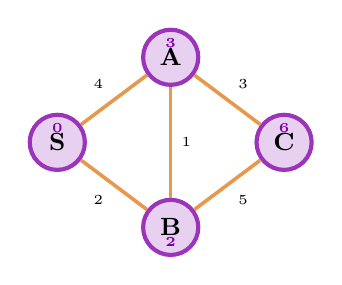
\begin{tikzpicture}[scale=0.72]
          \node[vnoDij,minimum size=7mm](s) at (0.0,2.5){S};
          \node[vnoDij,minimum size=7mm](a) at (2.0,4.0){A};
          \node[vnoDij,minimum size=7mm](b) at (2.0,1.0){B};
          \node[vnoDij,minimum size=7mm](c) at (4.0,2.5){C};
          \draw[epeso](s)--(a) node[midway,above left,font=\tiny]{4};
          \draw[epeso](s)--(b) node[midway,below left,font=\tiny]{2};
          \draw[epeso](a)--(c) node[midway,above right,font=\tiny]{3};
          \draw[epeso](b)--(a) node[midway,right,font=\tiny]{1};
          \draw[epeso](b)--(c) node[midway,below right,font=\tiny]{5};
          % Distâncias finais
          \node[pqColor,font=\tiny\bfseries,above] at (s){0};
          \node[pqColor,font=\tiny\bfseries,above] at (a){3};
          \node[pqColor,font=\tiny\bfseries,below] at (b){2};
          \node[pqColor,font=\tiny\bfseries,above] at (c){6};
        \end{tikzpicture}

        \begin{tabular}{ccccc}
          \toprule
          \textbf{Passo} & \textbf{v} & \textbf{dist[S]} & \textbf{dist[A]} & \textbf{dist[B]}\\
          \midrule
          init & --- & 0 & $\infty$ & $\infty$\\
          1 & S & 0 & 4 & 2\\
          2 & B & 0 & \textbf{3} & 2\\
          3 & A & 0 & 3 & 2\\
          4 & C & \multicolumn{3}{c}{dist[C]=6}\\
          \bottomrule
        \end{tabular}
      \end{tcolorbox}
  \end{columns}
\end{frame}

% ─────────────────────────────────────────────────────────────
%  DIJKSTRA — CÓDIGO COMPLETO
% ─────────────────────────────────────────────────────────────
\begin{frame}[fragile,shrink=3]{Dijkstra --- Código Completo em C++}
  \begin{columns}[t]
    \column{0.57\textwidth}
      \begin{tcolorbox}[caixaCodigo]
        \begin{lstlisting}[style=cppsmall]
#include <bits/stdc++.h>
using namespace std;
typedef pair<int,int> pii;
const int INF = 1e9;

// adj[v] = lista de {vizinho, peso}
vector<int> dijkstra(int s, int N,
    vector<vector<pii>>& adj) {

    vector<int> dist(N+1, INF);
    // min-heap: {distancia, no}
    priority_queue<pii, vector<pii>,
                   greater<pii>> pq;

    dist[s] = 0;
    pq.push({0, s});

    while (!pq.empty()) {
        auto [d, v] = pq.top(); pq.pop();

        // Entrada desatualizada? Ignora.
        if (d > dist[v]) continue;

        for (auto [peso, u] : adj[v]) {
            if (dist[v] + peso < dist[u]) {
                dist[u] = dist[v] + peso;
                pq.push({dist[u], u});
            }
        }
    }
    return dist; // dist[v] = custo minimo s->v
}

int main() {
    int N, M; cin >> N >> M;
    vector<vector<pii>> adj(N+1);
    for (int i = 0; i < M; i++) {
        int u, v, w; cin >> u >> v >> w;
        adj[u].push_back({w, v});
        adj[v].push_back({w, u}); // bidirecional
    }
    auto dist = dijkstra(1, N, adj);
    for (int i = 1; i <= N; i++)
        cout << "dist[" << i << "] = "
             << (dist[i]==INF ? -1 : dist[i])
             << "\n";
}
        \end{lstlisting}
      \end{tcolorbox}
    \column{0.41\textwidth}
      \begin{tcolorbox}[caixaRoxa,title={Por que min-heap com pares?}]
        \footnotesize
        \texttt{priority\_queue} é max-heap\\por padrão. Usamos\\
        \texttt{greater<pii>} para min-heap.\\[4pt]
        Par \texttt{\{distância, nó\}}:\\
        comparação pelo 1º campo\\
        $\Rightarrow$ menor distância sai primeiro.
      \end{tcolorbox}
      \vspace{0.07cm}
      \begin{tcolorbox}[caixaVerde,title={Complexidade}]
        \footnotesize
        \textbf{Tempo:} O((V+E) log V)\\
        Cada aresta: 1 push O(log V)\\
        Cada vértice: 1 pop O(log V)\\[3pt]
        \textbf{Espaço:} O(V+E)
      \end{tcolorbox}
      \vspace{0.07cm}
      \begin{tcolorbox}[caixaVermelho,title={Cuidados}]
        \footnotesize
        \textbf{Não funciona} com pesos\\negativos. Use \textbf{Bellman-Ford}.\\[3pt]
        Entradas \textbf{desatualizadas} na PQ:\\
        sempre checar\\
        \texttt{if (d > dist[v]) continue;}\\[3pt]
        \textbf{INF:} use \texttt{1e9} (int) ou\\
        \texttt{1e18} (long long)
      \end{tcolorbox}
      \vspace{0.07cm}
      \begin{tcolorbox}[caixaAmarelo,title={Reconstruir caminho}]
        \footnotesize
        Adicione \texttt{vector<int> prev(N+1,-1)}\\
        e \texttt{prev[u]=v} ao relaxar.\\
        Trace de volta de destino até s.
      \end{tcolorbox}
  \end{columns}
\end{frame}

% =============================================================
%  COMPARAÇÃO BFS vs DFS vs DIJKSTRA
% =============================================================
\begin{frame}{BFS vs DFS vs Dijkstra --- Comparação}
  \begin{tcolorbox}[caixaAzul,title={Tabela Comparativa}]
    \centering\footnotesize
    \begin{tabular}{lcccl}
      \toprule
      \textbf{Algoritmo} & \textbf{Estrutura} & \textbf{Complexidade} &
      \textbf{Menor caminho?} & \textbf{Quando usar}\\
      \midrule
      BFS       & Queue     & O(V+E)          & Sim (sem pesos)  & Grafos sem peso, labirintos\\
      DFS       & Stack/rec.& O(V+E)          & Não              & Componentes, ciclos, DFS-tree\\
      Dijkstra  & Min-heap  & O((V+E) log V)  & Sim (pesos $\ge$ 0) & Grafos com pesos positivos\\
      \bottomrule
    \end{tabular}
  \end{tcolorbox}
  \vspace{0.1cm}
  \begin{columns}[t]
    \column{0.32\textwidth}
      \begin{tcolorbox}[caixaLaranja,title={Use BFS quando}]
        \begin{itemize}\footnotesize
          \item Pesos = 1 (ou sem peso)
          \item Grade/labirinto
          \item Menor nº de passos
          \item Propagação em ``onda''
        \end{itemize}
      \end{tcolorbox}
    \column{0.32\textwidth}
      \begin{tcolorbox}[caixaDfs,title={Use DFS quando}]
        \begin{itemize}\footnotesize
          \item Contar componentes
          \item Detectar ciclos
          \item Ordenação topológica
          \item Backtracking
        \end{itemize}
      \end{tcolorbox}
    \column{0.32\textwidth}
      \begin{tcolorbox}[caixaRoxa,title={Use Dijkstra quando}]
        \begin{itemize}\footnotesize
          \item Pesos diferentes
          \item Pesos $\ge 0$
          \item Mapa com distâncias
          \item Menor custo de rota
        \end{itemize}
      \end{tcolorbox}
  \end{columns}
\end{frame}

% =============================================================
%  DIVISOR CLÁSSICOS
% =============================================================
{
\setbeamertemplate{footline}{}
\begin{frame}[noframenumbering]
  \centering\vspace{1.2cm}
  {\fontsize{38}{46}\selectfont\bfseries\color{gemaBlue} 6}\par
  \vspace{0.25cm}
  {\Large\color{mstColor}\bfseries Conteúdos Clássicos}\par
  \vspace{0.15cm}
  {\color{gray}\small MST $\cdot$ Fluxo Máximo $\cdot$ Ordenação Topológica $\cdot$ Árvores}
\end{frame}
}

% ─────────────────────────────────────────────────────────────
%  MST
% ─────────────────────────────────────────────────────────────
\begin{frame}[fragile]{MST --- Árvore Geradora Mínima}
  \begin{columns}[c]
    \column{0.47\textwidth}
      \begin{tcolorbox}[caixaAzul,title={O que é MST?}]
        \small
        Dado grafo conectado com pesos,
        encontrar subconjunto de arestas que
        \textbf{conecta todos os vértices}
        com \textbf{custo total mínimo}.
      \end{tcolorbox}
      \vspace{0.08cm}
      \begin{tcolorbox}[caixaGrafo,title={Kruskal}]
        \footnotesize
        1. Ordena arestas por peso\\
        2. Para cada aresta $(u,v,w)$:\\
        \quad Se $u$ e $v$ em componentes diferentes:\\
        \quad\quad adiciona à MST (usa \textbf{DSU/Union-Find})\\[3pt]
        \textbf{Complexidade:} O(E log E)\\
        \textbf{Melhor para:} grafos esparsos
      \end{tcolorbox}
      \vspace{0.08cm}
      \begin{tcolorbox}[caixaDfs,title={Prim}]
        \footnotesize
        Expande a MST a partir de um vértice,\\
        sempre adicionando a aresta de menor\\
        peso que conecta a MST a um novo nó.\\[3pt]
        Usa \textbf{priority\_queue} (igual ao Dijkstra)\\
        \textbf{Complexidade:} O((V+E) log V)
      \end{tcolorbox}
    \column{0.51\textwidth}
      \centering
      \begin{tcolorbox}[caixaAmarelo,title={Exemplo MST}]
        \centering\footnotesize
        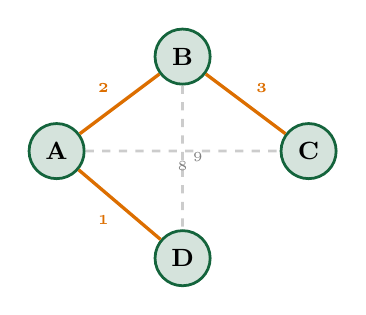
\begin{tikzpicture}[scale=0.80]
          \node[vnoG,minimum size=7mm](a) at (0.0,2.5){A};
          \node[vnoG,minimum size=7mm](b) at (2.0,4.0){B};
          \node[vnoG,minimum size=7mm](c) at (4.0,2.5){C};
          \node[vnoG,minimum size=7mm](d) at (2.0,0.8){D};
          % Arestas não-MST
          \draw[gray!40,dashed,line width=1pt]
            (a)--(c) node[midway,below,font=\tiny,gray]{8}
            (b)--(d) node[midway,right,font=\tiny,gray]{9};
          % Arestas MST (destacadas)
          \draw[gemaOrange,very thick]
            (a)--(b) node[midway,above left,font=\bfseries\tiny,gemaOrange]{2};
          \draw[gemaOrange,very thick]
            (b)--(c) node[midway,above right,font=\bfseries\tiny,gemaOrange]{3};
          \draw[gemaOrange,very thick]
            (d)--(a) node[midway,below left,font=\bfseries\tiny,gemaOrange]{1};
        \end{tikzpicture}\\[4pt]
        MST (laranja): peso total = 1+2+3 = \textbf{6}\\
        Arestas descartadas (cinza): 8 e 9
      \end{tcolorbox}
      \vspace{0.08cm}
      \begin{tcolorbox}[caixaVerde,title={Aplicações}]
        \footnotesize
        Redes de cabos com custo mínimo\\
        Clustering (K-MST)\\
        Problemas de conectividade\\
        \textbf{OBI:} ``conectar cidades com menor custo''
      \end{tcolorbox}
  \end{columns}
\end{frame}

% ─────────────────────────────────────────────────────────────
%  KRUSKAL — CÓDIGO RESUMIDO
% ─────────────────────────────────────────────────────────────
\begin{frame}[fragile,shrink=2]{Kruskal + DSU (Union-Find)}
  \begin{columns}[t]
    \column{0.58\textwidth}
      \begin{tcolorbox}[caixaCodigo]
        \begin{lstlisting}[style=cppsmall]
#include <bits/stdc++.h>
using namespace std;

// DSU (Disjoint Set Union)
struct DSU {
    vector<int> pai, rank_;
    DSU(int n) : pai(n+1), rank_(n+1, 0) {
        iota(pai.begin(), pai.end(), 0);
    }
    int find(int x) {
        if (pai[x] != x)
            pai[x] = find(pai[x]); // path compression
        return pai[x];
    }
    bool unite(int x, int y) {
        x = find(x); y = find(y);
        if (x == y) return false; // mesmo componente
        if (rank_[x] < rank_[y]) swap(x, y);
        pai[y] = x;
        if (rank_[x] == rank_[y]) rank_[x]++;
        return true;
    }
};

int kruskal(int N, vector<tuple<int,int,int>>& edges) {
    sort(edges.begin(), edges.end()); // por peso
    DSU dsu(N);
    int custo = 0, count = 0;
    for (auto [w, u, v] : edges) {
        if (dsu.unite(u, v)) {
            custo += w;
            count++;
            if (count == N-1) break; // MST completa
        }
    }
    return custo;
}
        \end{lstlisting}
      \end{tcolorbox}
    \column{0.40\textwidth}
      \begin{tcolorbox}[caixaGrafo,title={DSU (Union-Find)}]
        \footnotesize
        Estrutura para \textbf{conjuntos disjuntos}.\\[3pt]
        \texttt{find(x)}: raiz do conjunto de x\\
        \texttt{unite(x,y)}: une dois conjuntos\\[3pt]
        Com \textbf{path compression} + \textbf{rank}:\\
        quase O(1) por operação $\approx$ O($\alpha(n)$)
      \end{tcolorbox}
      \vspace{0.07cm}
      \begin{tcolorbox}[caixaAmarelo,title={Invariante Kruskal}]
        \footnotesize
        Uma MST com $N$ vértices\\
        tem exatamente \textbf{N-1 arestas}.\\[3pt]
        Quando \texttt{count == N-1}:\\
        a MST está completa!
      \end{tcolorbox}
      \vspace{0.07cm}
      \begin{tcolorbox}[caixaVerde,title={Complexidade}]
        \footnotesize
        Ordenar: O(E log E)\\
        DSU: O(E $\alpha$(N)) $\approx$ O(E)\\[3pt]
        \textbf{Total: O(E log E)}
      \end{tcolorbox}
      \vspace{0.07cm}
      \begin{tcolorbox}[caixaVermelho,title={Atenção}]
        \footnotesize
        \texttt{tuple<int,int,int>}:\\
        primeiro campo = peso\\
        (para sort funcionar certo)
      \end{tcolorbox}
  \end{columns}
\end{frame}

% ─────────────────────────────────────────────────────────────
%  ORDENAÇÃO TOPOLÓGICA
% ─────────────────────────────────────────────────────────────
\begin{frame}[fragile]{Ordenação Topológica (Toposort)}
  \begin{columns}[t]
    \column{0.50\textwidth}
      \begin{tcolorbox}[caixaAzul,title={O que é?}]
        \small
        Dado um \textbf{DAG} (grafo dirigido acíclico),\\
        ordenar os vértices de forma que\\
        para toda aresta $(u \to v)$,\\
        $u$ aparece \textbf{antes} de $v$.
      \end{tcolorbox}
      \vspace{0.07cm}
      \begin{tcolorbox}[caixaGrafo,title={Algoritmo de Kahn (BFS)}]
        \footnotesize
        1. Calcular \textbf{in-degree} de cada vértice\\
        2. Enfileirar vértices com in-degree = 0\\
        3. Enquanto queue não vazia:\\
        \quad Retirar $v$, adicionar à ordem\\
        \quad Para cada $u$ vizinho de $v$:\\
        \quad\quad \texttt{in[u]--}\\
        \quad\quad Se \texttt{in[u] == 0}: enfileirar $u$\\[3pt]
        Se \texttt{ordem.size() $\neq$ N}: \textbf{tem ciclo!}
      \end{tcolorbox}
      \vspace{0.07cm}
      \begin{tcolorbox}[caixaAmarelo,title={Aplicações}]
        \footnotesize
        Dependências (compilação, pacotes)\\
        Sequência de tarefas\\
        Pré-requisitos de cursos\\
        Programação dinâmica em DAG
      \end{tcolorbox}
    \column{0.48\textwidth}
      \begin{tcolorbox}[caixaCodigo]
        \begin{lstlisting}[style=cppsmall]
vector<int> toposort(int N,
    vector<vector<int>>& adj) {

    vector<int> indegree(N+1, 0);
    for (int v = 1; v <= N; v++)
        for (int u : adj[v])
            indegree[u]++;

    queue<int> q;
    for (int v = 1; v <= N; v++)
        if (indegree[v] == 0) q.push(v);

    vector<int> ordem;
    while (!q.empty()) {
        int v = q.front(); q.pop();
        ordem.push_back(v);
        for (int u : adj[v]) {
            indegree[u]--;
            if (indegree[u] == 0)
                q.push(u);
        }
    }
    // Se ordem.size() != N: ciclo!
    return ordem;
}
        \end{lstlisting}
      \end{tcolorbox}
      \begin{tcolorbox}[caixaVerde,title={Complexidade}]
        \footnotesize
        \textbf{Tempo:} O(V + E)\\
        \textbf{Espaço:} O(V)
      \end{tcolorbox}
    \end{columns}
\end{frame}

% ─────────────────────────────────────────────────────────────
%  FLUXO MÁXIMO
% ─────────────────────────────────────────────────────────────
\begin{frame}{Fluxo Máximo --- Ideia Geral}
  \begin{columns}[c]
    \column{0.50\textwidth}
      \begin{tcolorbox}[caixaAzul,title={Problema}]
        \small
        Dado grafo dirigido com \textbf{capacidades},
        encontrar o \textbf{fluxo máximo} que pode
        ser enviado da \textbf{fonte} S ao \textbf{sumidouro} T.
      \end{tcolorbox}
      \vspace{0.08cm}
      \begin{tcolorbox}[caixaGrafo,title={Ford-Fulkerson (ideia)}]
        \footnotesize
        1. Enquanto existe \textbf{caminho aumentante}\\
        \quad (S $\to$ T com capacidade residual $>$ 0):
        \begin{itemize}\scriptsize
          \item Encontrar caminho P (BFS = Edmonds-Karp)
          \item Achar gargalo = mínima capacidade em P
          \item Enviar fluxo pelo caminho
          \item Atualizar capacidades residuais
        \end{itemize}
      \end{tcolorbox}
      \vspace{0.08cm}
      \begin{tcolorbox}[caixaAmarelo,title={Complexidade}]
        \footnotesize
        \textbf{Ford-Fulkerson:} O(E $\cdot$ |fluxo máx.|)\\
        \textbf{Edmonds-Karp} (BFS): O(V $\cdot$ E$^2$)\\
        \textbf{Dinic:} O(V$^2$ $\cdot$ E) --- mais rápido
      \end{tcolorbox}
      \vspace{0.08cm}
      \begin{tcolorbox}[caixaVerde,title={Teorema min-corte max-fluxo}]
        \footnotesize
        Fluxo máximo = corte mínimo.\\
        Corte = partição de V em S-side e T-side.
      \end{tcolorbox}
    \column{0.48\textwidth}
      \centering
      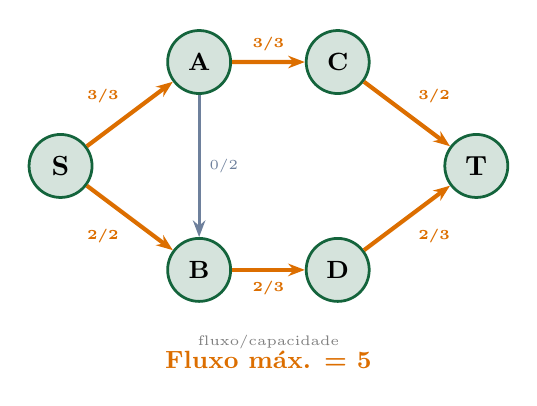
\begin{tikzpicture}[scale=0.88]
        \node[vnoG,minimum size=8mm,font=\bfseries](s)  at (0.0,2.0){S};
        \node[vnoG,minimum size=8mm](a) at (2.0,3.5){A};
        \node[vnoG,minimum size=8mm](b) at (2.0,0.5){B};
        \node[vnoG,minimum size=8mm](c) at (4.0,3.5){C};
        \node[vnoG,minimum size=8mm](d) at (4.0,0.5){D};
        \node[vnoG,minimum size=8mm,font=\bfseries](t) at (6.0,2.0){T};
        % Arestas com capacidade/fluxo
        \draw[edir,gemaOrange,line width=1.5pt](s)--(a)
          node[midway,above left,font=\tiny\bfseries]{3/3};
        \draw[edir,gemaOrange,line width=1.5pt](s)--(b)
          node[midway,below left,font=\tiny\bfseries]{2/2};
        \draw[edir,gemaBlue!60,line width=1pt](a)--(b)
          node[midway,right,font=\tiny]{0/2};
        \draw[edir,gemaOrange,line width=1.5pt](a)--(c)
          node[midway,above,font=\tiny\bfseries]{3/3};
        \draw[edir,gemaOrange,line width=1.5pt](b)--(d)
          node[midway,below,font=\tiny\bfseries]{2/3};
        \draw[edir,gemaOrange,line width=1.5pt](c)--(t)
          node[midway,above right,font=\tiny\bfseries]{3/2};
        \draw[edir,gemaOrange,line width=1.5pt](d)--(t)
          node[midway,below right,font=\tiny\bfseries]{2/3};
        \node[font=\tiny,gray,below] at (3.0,-0.3){fluxo/capacidade};
        \node[font=\bfseries\small,gemaOrange] at (3.0,-0.8){Fluxo máx. = 5};
      \end{tikzpicture}
      \vspace{0.08cm}
      \begin{tcolorbox}[caixaVermelho,title={Aplicações}]
        \footnotesize
        Redes de computadores\\
        Matching bipartido\\
        Corte mínimo em grafos\\
        Problemas de distribuição
      \end{tcolorbox}
  \end{columns}
\end{frame}

% ─────────────────────────────────────────────────────────────
%  ÁRVORES
% ─────────────────────────────────────────────────────────────
\begin{frame}{Árvores --- Conceito e Propriedades}
  \begin{columns}[c]
    \column{0.47\textwidth}
      \begin{tcolorbox}[caixaAzul,title={Definição}]
        \small
        Uma \textbf{árvore} é um grafo \textbf{conexo acíclico}.\\[4pt]
        Equivalentemente: grafo com $N$ vértices\\
        e exatamente $N-1$ arestas, conexo.
      \end{tcolorbox}
      \vspace{0.08cm}
      \begin{tcolorbox}[caixaGrafo,title={Propriedades}]
        \begin{itemize}\footnotesize
          \item Entre qualquer par de vértices\\
                existe \textbf{exatamente 1 caminho}
          \item Remover qualquer aresta:\\
                desconecta o grafo
          \item Adicionar qualquer aresta:\\
                cria exatamente 1 ciclo
          \item Uma árvore com $N$ vértices\\
                tem $N-1$ arestas
        \end{itemize}
      \end{tcolorbox}
      \vspace{0.08cm}
      \begin{tcolorbox}[caixaAmarelo,title={Relação com grafos}]
        \footnotesize
        MST é uma árvore geradora.\\
        Árvore de BFS = subgrafos de BFS.\\
        Todo grafo conexo tem uma árvore\\
        geradora (spanning tree).
      \end{tcolorbox}
    \column{0.51\textwidth}
      \centering
      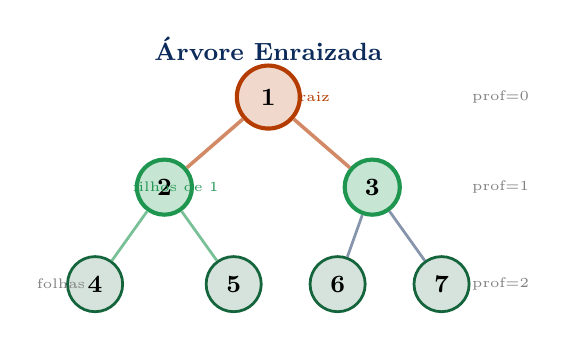
\begin{tikzpicture}[scale=0.88]
        % Árvore enraizada
        \node[font=\bfseries\small,gemaBlue] at (3.0,5.2){Árvore Enraizada};
        \node[vnoDFS,minimum size=8mm](r)  at (3.0,4.5){1};
        \node[vnoVis,minimum size=7mm](n2) at (1.5,3.2){2};
        \node[vnoVis,minimum size=7mm](n3) at (4.5,3.2){3};
        \node[vnoG,minimum size=7mm](n4) at (0.5,1.8){4};
        \node[vnoG,minimum size=7mm](n5) at (2.5,1.8){5};
        \node[vnoG,minimum size=7mm](n6) at (4.0,1.8){6};
        \node[vnoG,minimum size=7mm](n7) at (5.5,1.8){7};
        \draw[dfsColor!60,line width=1.3pt](r)--(n2)(r)--(n3);
        \draw[nodeGreen!60,line width=1pt](n2)--(n4)(n2)--(n5);
        \draw[gemaBlue!50,line width=1pt](n3)--(n6)(n3)--(n7);
        % Anotações
        \node[font=\tiny,dfsColor,right] at (3.3,4.5){raiz};
        \node[font=\tiny,nodeGreen,right] at (0.9,3.2){filhos de 1};
        \node[font=\tiny,gray,left] at (0.5,1.8){folhas};
        % Profundidades
        \node[font=\tiny,gray,right] at (5.8,4.5){prof=0};
        \node[font=\tiny,gray,right] at (5.8,3.2){prof=1};
        \node[font=\tiny,gray,right] at (5.8,1.8){prof=2};
      \end{tikzpicture}
      \vspace{0.05cm}
      \begin{tcolorbox}[caixaVermelho,title={Terminologia}]
        \footnotesize
        \textbf{Raiz}: vértice sem pai\\
        \textbf{Folha}: vértice sem filhos\\
        \textbf{Profundidade}: dist. da raiz\\
        \textbf{Altura}: profundidade máxima\\
        \textbf{Subárvore}: nó + descendentes
      \end{tcolorbox}
  \end{columns}
\end{frame}

% =============================================================
%  DIVISOR DICAS
% =============================================================
{
\setbeamertemplate{footline}{}
\begin{frame}[noframenumbering]
  \centering\vspace{1.2cm}
  {\fontsize{38}{46}\selectfont\bfseries\color{gemaBlue} 7}\par
  \vspace{0.25cm}
  {\Large\color{gemaOrange}\bfseries Dicas de Programação Competitiva}\par
  \vspace{0.15cm}
  {\color{gray}\small Identificar $\cdot$ Erros comuns $\cdot$ Palavras-chave}
\end{frame}
}

% ─────────────────────────────────────────────────────────────
%  COMO IDENTIFICAR
% ─────────────────────────────────────────────────────────────
\begin{frame}{Como Identificar o Algoritmo Certo}
  \begin{columns}[t]
    \column{0.47\textwidth}
      \begin{block}{Palavras-chave: grafo}
        \begin{itemize}\footnotesize
          \item ``Cidades e estradas''
          \item ``Rede de computadores''
          \item ``Dependências entre tarefas''
          \item ``Labirinto'', ``grade NxM''
          \item ``Amizades'', ``conexões''
          \item ``Componentes'', ``grupos''
        \end{itemize}
      \end{block}
      \vspace{0.1cm}
      \begin{tcolorbox}[caixaLaranja,title={Sinais de BFS}]
        \footnotesize
        ``Menor número de passos''\\
        ``Mínimo de movimentos''\\
        ``Distância mínima'' (sem pesos)\\
        Grade com custo = 1 por célula
      \end{tcolorbox}
      \vspace{0.1cm}
      \begin{tcolorbox}[caixaDfs,title={Sinais de DFS}]
        \footnotesize
        ``Componentes conexas''\\
        ``Existe caminho entre A e B?''\\
        ``Ciclos no grafo''\\
        ``Ordenação de dependências'' (DAG)
      \end{tcolorbox}
    \column{0.50\textwidth}
      \begin{tcolorbox}[caixaRoxa,title={Sinais de Dijkstra}]
        \footnotesize
        ``Menor custo'' com pesos $\ge$ 0\\
        ``Mínima distância'' em mapa com km\\
        ``Caminho mais barato''\\
        Pesos diferentes por aresta
      \end{tcolorbox}
      \vspace{0.1cm}
      \begin{tcolorbox}[caixaGrafo,title={Sinais de MST}]
        \footnotesize
        ``Conectar tudo com custo mínimo''\\
        ``Rede de distribuição elétrica''\\
        ``Menor conjunto de estradas\\
        que conecta todas as cidades''
      \end{tcolorbox}
      \vspace{0.1cm}
      \begin{tcolorbox}[caixaAmarelo,title={Pergunta mágica}]
        \footnotesize
        \textbf{Sem pesos?} $\to$ BFS\\
        \textbf{Com pesos $\ge$ 0?} $\to$ Dijkstra\\
        \textbf{Com pesos negativos?} $\to$ Bellman-Ford\\
        \textbf{Conectar tudo?} $\to$ MST (Kruskal/Prim)\\
        \textbf{Explorar/componentes?} $\to$ DFS\\
        \textbf{Dependências?} $\to$ Toposort
      \end{tcolorbox}
  \end{columns}
\end{frame}

% ─────────────────────────────────────────────────────────────
%  ERROS COMUNS
% ─────────────────────────────────────────────────────────────
\begin{frame}[fragile]{Erros Comuns em Problemas de Grafo}
  \begin{columns}[t]
    \column{0.48\textwidth}
      \begin{alertblock}{Erros de Implementação}
        \begin{itemize}\footnotesize
          \item Esquecer de checar \texttt{!vis[u]} no BFS/DFS
          \item Usar \texttt{vector} com tamanho errado (off-by-one)
          \item Não limpar \texttt{vis}/\texttt{dist} entre queries
          \item Usar \texttt{int} quando precisa \texttt{long long}\\
                (somas de pesos podem estourar)
          \item Esquecer \texttt{if (d > dist[v]) continue;}\\
                no Dijkstra
        \end{itemize}
      \end{alertblock}
      \vspace{0.1cm}
      \begin{tcolorbox}[caixaVermelho,title={Armadilha: grafos desconexos}]
        \footnotesize
        \textbf{Sempre} rode BFS/DFS de\\
        \textbf{todos} os vértices não visitados\\
        se o grafo pode ser desconexo!\\[3pt]
        \begin{lstlisting}[style=cppsmall,numbers=none]
for (int v=1; v<=N; v++)
    if (!vis[v]) bfs(v, adj);
        \end{lstlisting}
      \end{tcolorbox}
    \column{0.48\textwidth}
      \begin{tcolorbox}[caixaAmarelo,title={Armadilha: índice 0 vs 1}]
        \footnotesize
        Decidir \textbf{antes} de codar:\\
        vértices de 0 a N-1 ou de 1 a N?\\[3pt]
        \begin{lstlisting}[style=cppsmall,numbers=none]
// Padrao recomendado: 1-indexed
vector<vector<int>> adj(N+1);
vector<bool> vis(N+1, false);
vector<int> dist(N+1, INF);
        \end{lstlisting}
      \end{tcolorbox}
      \vspace{0.08cm}
      \begin{tcolorbox}[caixaGrafo,title={Verificar antes de submeter}]
        \begin{itemize}\footnotesize
          \item Grafo pode ser desconexo?
          \item Arestas são bidirecionais?
          \item Pesos podem ser negativos?
          \item Pode haver arestas múltiplas?
          \item Pode haver self-loops?
          \item $N$ e $M$ cabem na memória?
        \end{itemize}
      \end{tcolorbox}
      \vspace{0.08cm}
      \begin{tcolorbox}[caixaVerde,title={Dica: template padrão}]
        \footnotesize
        \begin{lstlisting}[style=cppsmall,numbers=none]
int N, M;
cin >> N >> M;
vector<vector<int>> adj(N+1);
for (int i=0; i<M; i++) {
    int u, v; cin >> u >> v;
    adj[u].push_back(v);
    adj[v].push_back(u);
}
        \end{lstlisting}
      \end{tcolorbox}
  \end{columns}
\end{frame}

% ─────────────────────────────────────────────────────────────
%  RESUMO GERAL
% ─────────────────────────────────────────────────────────────
\begin{frame}[shrink=2]{Resumo Geral}
  \begin{columns}[t]
    \column{0.32\textwidth}
      \begin{block}{Representação}
        \begin{itemize}\footnotesize
          \item Lista adj: O(V+E), padrão
          \item Matriz: O(V$^2$), $N \le 1000$
          \item Lista arestas: Kruskal
        \end{itemize}
      \end{block}
      \vspace{0.05cm}
      \begin{block}{BFS}
        \begin{itemize}\footnotesize
          \item Queue, O(V+E)
          \item Menor caminho s/ peso
          \item Grid, labirinto, ondas
        \end{itemize}
      \end{block}
    \column{0.32\textwidth}
      \begin{block}{DFS}
        \begin{itemize}\footnotesize
          \item Recursivo/Iterativo
          \item O(V+E)
          \item Componentes, ciclos
        \end{itemize}
      \end{block}
      \vspace{0.05cm}
      \begin{block}{Dijkstra}
        \begin{itemize}\footnotesize
          \item Min-heap, O((V+E)log V)
          \item Menor caminho c/ pesos $\ge$ 0
          \item \texttt{priority\_queue<pii,...>}
        \end{itemize}
      \end{block}
    \column{0.32\textwidth}
      \begin{block}{Clássicos}
        \begin{itemize}\footnotesize
          \item MST: Kruskal + DSU, Prim
          \item Toposort: Kahn (BFS)
          \item Fluxo: Ford-Fulkerson
          \item Árvores: $N$ vértices, $N$-1 arestas
        \end{itemize}
      \end{block}
    \end{columns}
  \vspace{0.10cm}
  \begin{columns}[t]
    \column{0.50\textwidth}
      % \begin{tcolorbox}[caixaVerde,title={Problemas para Praticar}]
      %   \footnotesize
      %   \textbf{BFS:} CF 1891B, NEPS Labirinto\\
      %   \textbf{DFS:} CF 1037D, componentes conexas\\
      %   \textbf{Dijkstra:} CF 20C, SPOJ SHPATH\\
      %   \textbf{MST:} CF 1468C, NEPS estradas\\
      %   \textbf{Toposort:} CF 510C, OBI tarefas
      % \end{tcolorbox}
    \column{0.48\textwidth}
      \begin{tcolorbox}[caixaAzul,title={Templates Mentais}]
        \footnotesize
        \textbf{BFS:}
        \texttt{queue<int> q; vis[s]=true; q.push(s);}\\[2pt]
        \textbf{DFS:}
        \texttt{void dfs(int v)\{vis[v]=true;\}}\\[2pt]
        \textbf{Dijkstra:}
        \texttt{priority\_queue<pii,vector<pii>,greater<pii>> pq;}\\
        \texttt{dist[s]=0; pq.push(\{0,s\});}\\[2pt]
        \textbf{Kruskal:}
        \texttt{sort(edges); DSU dsu(N);}
      \end{tcolorbox}
  \end{columns}
\end{frame}

% ─────────────────────────────────────────────────────────────
%  SLIDE FINAL
% ─────────────────────────────────────────────────────────────
% ─────────────────────────────────────────────────────────────
%  SLIDE FINAL
% ─────────────────────────────────────────────────────────────
{
\setbeamertemplate{footline}{}
\begin{frame}[noframenumbering]
  \centering\vspace{0.1cm}
  \begin{columns}[c]
    \column{0.28\textwidth}
      \centering
\includegraphics[width=0.65\linewidth]{logo.png}
    \column{0.40\textwidth}
      \centering
      {\large\color{gemaBlue}\bfseries Bons estudos\\e boa prova!}\par
      \vspace{0.12cm}
      {\small\color{gemaCyan} GEMA --- Maratonas de Programação}\par
      \vspace{0.12cm}
      % {\footnotesize\color{gray} Proxima aula: Grafos --- BFS/DFS avancado}
    \column{0.28\textwidth}
      \centering
\includegraphics[width=0.65\linewidth]{logo_obi.png}
  \end{columns}
  \vspace{0.2cm}
  % \begin{tcolorbox}[caixaAzul,title={Dica de Ouro},width=0.82\textwidth]
  %   \centering\small
  %   \textbf{Regra das 3 perguntas:}\\[4pt]
  %   ``Preciso do mais recente?'' $\to$ \textbf{Stack}\\
  %   ``Preciso do mais antigo?'' $\to$ \textbf{Queue}\\
  %   ``Preciso do mais importante?'' $\to$ \textbf{Priority Queue}
  % \end{tcolorbox}
  % \vspace{0.15cm}
  % \begin{tcolorbox}[caixaVerde,title={},width=0.80\textwidth]
  %   \centering\footnotesize
  %   \textbf{Pratique:} \texttt{codeforces.com} $\cdot$ \texttt{neps.com.br}
  %   $\cdot$ \texttt{cses.fi}\\[2pt]
  %   \textbf{Estude:} cp-algorithms.com $\cdot$ USACO Guide
  % \end{tcolorbox}
  \vspace{0.12cm}
  {\small\color{gray}\itshape
    ``A computação é o estudo dos Grafos''}
\end{frame}
}


\end{document}